\documentclass[11pt,oneside]{book}

\usepackage[T1]{fontenc}
\usepackage[utf8]{inputenc}
\usepackage{lmodern}
\usepackage{microtype}
\usepackage[a4paper,margin=25mm,headheight=14pt]{geometry}
\usepackage{mathtools,amssymb,bm}
\usepackage{siunitx}
\sisetup{per-mode=symbol,detect-all,range-phrase=--}
\usepackage{booktabs,longtable,tabularx,array,multirow}
\usepackage{graphicx,float,caption}
\usepackage{xcolor}
\usepackage{listings}
\usepackage{enumitem}
\usepackage{algorithm}
\usepackage{algpseudocode}
\usepackage{tikz}
\usetikzlibrary{arrows.meta,positioning,shapes.geometric,fit,calc,decorations.pathreplacing}
\usepackage{pgfplots}
\pgfplotsset{compat=1.18}
\usepackage{xurl}
\usepackage[colorlinks=true,linkcolor=blue!55!black,citecolor=green!40!black,urlcolor=blue!55!black]{hyperref}
\pdfstringdefDisableCommands{\def\code#1{#1}\def\file#1{#1}}
\usepackage[nameinlink,noabbrev]{cleveref}

\definecolor{codebg}{HTML}{F5F7FA}
\definecolor{codeframe}{HTML}{CBD2DC}
\definecolor{codeblue}{HTML}{174A7E}
\definecolor{codegreen}{HTML}{276749}
\lstdefinestyle{study}{
  backgroundcolor=\color{codebg},
  frame=single,rulecolor=\color{codeframe},
  basicstyle=\ttfamily\footnotesize,
  keywordstyle=\color{codeblue}\bfseries,
  commentstyle=\color{codegreen},
  stringstyle=\color{red!55!black},
  numbers=left,numberstyle=\tiny\color{gray},numbersep=8pt,
  breaklines=true,breakatwhitespace=false,
  showstringspaces=false,tabsize=4,columns=fullflexible,
  keepspaces=true,captionpos=b
}
\lstset{style=study}

\setcounter{tocdepth}{2}
\setcounter{secnumdepth}{3}
\setlist{nosep,leftmargin=*}
\allowdisplaybreaks

\newcommand{\R}{\mathbb{R}}
\newcommand{\SO}{\mathrm{SO}(3)}
\newcommand{\SE}{\mathrm{SE}(3)}
\newcommand{\Trans}{\,{}^{A}\!T_{B}}
\newcommand{\qvec}{\bm{q}}
\newcommand{\pvec}{\bm{p}}
\DeclareRobustCommand{\file}[1]{\path{#1}}
\DeclareRobustCommand{\code}[1]{\texttt{\detokenize{#1}}}
\newcommand{\sourcefile}[1]{\par\smallskip\noindent\textbf{Repository source: }\file{#1}\par\smallskip}
\newcommand{\verified}{\textsf{[verified in recorded project evidence]}}
\newcommand{\notretested}{\textsf{[source-inspected; not rerun in this guide task]}}

\title{Understanding the EN3563 GP7 Pick-and-Place Project\\[0.5em]
\large A Mathematical, Software, and Simulation Study Guide}
\author{Group members: [name and index number] \and [name and index number] \and [name and index number]}
\date{Prepared from repository branch \texttt{main}\\[0.4em]\today}

\begin{document}
\frontmatter
\maketitle
\chapter*{How to use this guide}
This is a study reference for explaining the actual GP7 project. It combines
textbook mathematics with implementation-specific facts, and labels the
boundary between them. The guide is deliberately more expansive than the
assignment report. The source of truth for runtime behavior is the repository's
ROS description, launch files, Python modules, controller YAML, SDF world, and
tests. Historical simulation outcomes are reported as recorded in
\file{docs/validation.md}; they are not claimed as new results from compiling
this guide.

Three evidence labels are used throughout:
\begin{description}
  \item[Verified in recorded project evidence] A result explicitly recorded in
  the repository's validation notes or produced by the independent checks
  documented in this guide.
  \item[Source-inspected, not rerun] A code path or configuration was examined,
  but no new Gazebo run was performed for this documentation task.
  \item[Theory] Mathematical explanation used to interpret the implementation;
  it is not necessarily an algorithm explicitly coded in the repository.
\end{description}

When presenting, explain the distinction between Box A and Box B precisely:
Box A is the fixed, large destination; Box B is the small object picked up.
Near-mode randomization changes Box B's pickup coordinates, not Box A.

\chapter*{Project provenance and scope}
The repository's authoritative branch for this guide is \texttt{main}, at the
state inspected for this document. The EN3563 assignment sheet is
\file{Task_sheet.pdf}. It asks for a four-or-more-DoF robot, coordinate frames,
a DH table, FK, IK, trajectory planning, velocity control, upright placement,
a report, and screen-recorded simulation video. The project uses a six-joint
GP7 URDF and a ROS 2/Gazebo implementation. The lecturer's later allowance for
a reachable Box A position was verbal, not text in the assignment sheet; this
guide makes no claim of written permission.

\tableofcontents
\listoffigures
\listoftables

\mainmatter
\chapter{Project Overview and Assignment}
\label{ch:overview}

\section{The engineering problem}
The EN3563 mini-project asks a group to implement a pick-and-place task with a
robot arm that has at least four degrees of freedom. The work is intentionally
end-to-end: model the robot, assign link coordinate frames, construct a DH
table, compute forward kinematics (FK), formulate inverse kinematics (IK),
plan a smooth trajectory, control the joints, keep the carried object upright,
and submit a report and screen-recorded demonstration. The supplied sheet
offers physical construction or a Gazebo simulation using the supplied
Yaskawa GP7 CAD. The simulation option explicitly allows a simplified gripper
because the supplied CAD robot does not include an end effector. It specifies
the robot at the origin, a large Box A of $0.30\times0.30\times0.20$ m, a
$0.05$ m cube Box B at a random reachable ground location, and Box B placement
at the center of Box A's top surface while preserving orientation
\cite{assignment}.

The implemented system is a ROS 2 and Gazebo Sim application around a six-axis
GP7 URDF. It is more than a static kinematics exercise: the launch code creates
a task-specific robot description, starts Gazebo and the controllers, chooses
Box B's pickup pose, and starts a Python node that plans, executes, monitors,
attaches, releases, and verifies the object.

\section{Original requirement, clarification, and implementation}
The original sheet places Box A at $(1,1,0)$ m. Relative to the robot base at
the origin, this has horizontal radius
\begin{equation}
  r_A=\sqrt{1^2+1^2}=\sqrt{2}\approx\SI{1.414}{m}.
  \label{eq:box-a-radius}
\end{equation}
The repository's engineering notes estimate an upper horizontal reach below
\SI{1.03}{m} for this robot model, before joint-limit constraints. Thus the
printed destination is not achievable in the implemented scene. After the
sheet was issued, the lecturer verbally clarified that a reachable Box A
location could be used. The implementation consequently fixes Box A's ground
position at $(0.55,0.35,0)$ m. This is a later verbal clarification; it is not
an amendment printed in the supplied sheet, and the group has no written
permission to claim.

The assignment's random reachable ground pose refers to the movable small
object, Box B. The project keeps Box A fixed while offering two Box B pickup
modes:
\begin{itemize}
  \item \textbf{Far mode}: numerical constrained optimization finds a
  maximum-radius, downward-facing grasp. The actual pickup is moved inward by
  a \SI{5}{mm} margin. It is optimized and deterministic, not random.
  \item \textbf{Near mode}: the launch file samples $x\sim U(0.50,0.60)$ and
  $y\sim U(-0.23,-0.15)$ using Python's seeded pseudorandom generator. With
  seed 7 the observed pose was $(0.532383276,-0.217932066,0.025)$ m. This
  changes Box B's pose only. A sampled point is not certified reachable solely
  by the sampling bounds; the path's IK preflight can reject an infeasible
  sample.
\end{itemize}
The fixed destination and the two pickup definitions are plotted in
\cref{fig:scene}.

\begin{figure}[htbp]
  \centering
  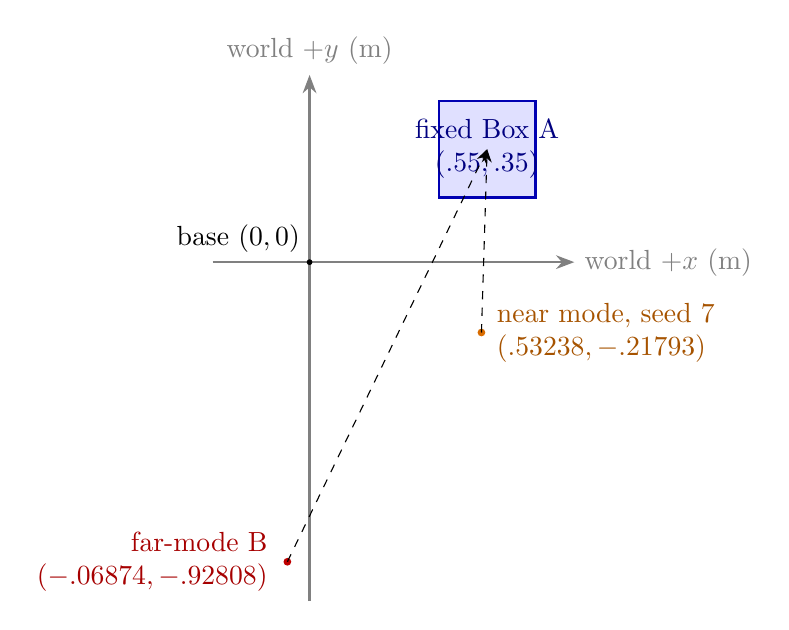
\begin{tikzpicture}[>=Stealth,scale=4.1]
  \draw[->,gray,thick] (-.30,0)--(.82,0) node[right]{world $+x$ (m)};
  \draw[->,gray,thick] (0,-1.05)--(0,.58) node[above]{world $+y$ (m)};
  \fill[blue!12] (.40,.20) rectangle (.70,.50);
  \draw[blue!70!black,thick] (.40,.20) rectangle (.70,.50);
  \node[blue!50!black,align=center] at (.55,.35){fixed Box A\\$(.55,.35)$};
  \fill[red!75!black] (-.06874,-.92808) circle (.012);
  \node[red!65!black,anchor=east,align=right] at (-.10,-.928){far-mode B\\$(-.06874,-.92808)$};
  \fill[orange!85!black] (.53238,-.21793) circle (.012);
  \node[orange!65!black,anchor=west,align=left] at (.55,-.218){near mode, seed 7\\$(.53238,-.21793)$};
  \fill[black] (0,0) circle (.009) node[above left]{base $(0,0)$};
  \draw[->,black,dashed] (-.06874,-.92808)--(.55,.35);
  \draw[->,black,dashed] (.53238,-.21793)--(.55,.35);
\end{tikzpicture}

  \caption{World-plane schematic of the fixed Box A and example Box B pickup
  locations. The vertical coordinate is suppressed; both pickup centers are
  at $z=0.025$ m.}
  \label{fig:scene}
\end{figure}

Box A's center is at $z=0.10$ m because its height is \SI{0.20}{m}. The target
center for Box B is
\begin{equation}
 \pvec_{B,d}=\begin{bmatrix}0.55&0.35&0.225\end{bmatrix}^{T}\si{m},
 \label{eq:place-target}
\end{equation}
which places the cube's lower face at $z=0.20$ m, the top of Box A. In the
actual path the tool lowers to $z=0.226$ m, releases about \SI{1}{mm} above
the target center, and the cube settles under gravity before final pose
measurement.

\section{Requirements and evidence status}
\begin{longtable}{p{.29\textwidth}p{.31\textwidth}p{.32\textwidth}}
\caption{Assignment requirement mapped to implementation and evidence.}\label{tab:req-map}\\
\toprule Requirement & Implementation & Status / limitation\\\midrule\endfirsthead
\toprule Requirement & Implementation & Status / limitation\\\midrule\endhead
At least four degrees of freedom & Six revolute GP7 joints & Implemented in URDF; all six are commanded.\\
Coordinate frame diagram & Standard-DH frames & Derived and independently compared to URDF FK; see \cref{ch:dh}.\\
DH table and FK & Standard DH table plus tool transform & 104-config comparison recorded; runtime FK itself parses URDF, not DH constants.\\
IK for target pose & Bounded SciPy least squares & Numerical solver with URDF limits; no analytic GP7 solver.\\
Smooth trajectory / velocity control & Quintic blend, sampled Cartesian IK, trajectory action & Joint-speed cap is sampled; no measured acceleration or jerk report.\\
Random reachable Box B & Seeded near-mode coordinate sampling & Seed 7 was tested; arbitrary samples are preflighted and can fail.\\
Box A position & Fixed $(0.55,0.35,0)$ m & Used under lecturer's subsequent verbal clarification; original sheet says $(1,1,0)$.\\
Upright object transfer & Fixed downward grasp rotation; orientation monitored from Gazebo pose samples & Successful simulation records; sampling is not a continuous-time proof.\\
Gripper / grasp & Adaptive mesh gripper and detachable fixed-joint plugin & Simulated close and attachment; no demonstrated frictional or physical grasp.\\
Report and video & This guide and prior report draft; recording checklist & Group member fields and a new screen recording remain submission work.\\
\bottomrule
\end{longtable}

\section{What is complete versus what remains}
The repo's validation notes record successful builds of all three ROS packages,
six offline regression tests, 104 DH-versus-URDF FK configurations, and
headless Gazebo far and seeded-near runs. The executed sequence included
approach, descent, close/attach, lift, transfer, placement, release, and
retreat. Those are simulation results with an idealized fixed-joint retention
mechanism. No physical robot run, force-based grasp, CAD equivalence study, or
submission video is in the repository evidence. Chapter 13 preserves the
recorded metrics and separates them from any verification done while preparing
this guide.

\section{Scope boundaries}
This guide explains both mathematical background and the actual choices made
in source. It does not claim the project uses MoveIt, an analytic IK solution,
a collision planner, physical sensors, force control, or calibrated link
inertias. None of those appears in the working task path. ROS 2, Gazebo, and
the Python stack interact, but the repository has no custom C++ source file;
the C++ plugins and controller implementations are supplied by installed ROS
and Gazebo packages.

\chapter{The Yaskawa GP7 Robot}
\label{ch:robot}

\section{Six revolute degrees of freedom}
A serial manipulator is a chain of rigid links connected by joints. A revolute
joint contributes one scalar coordinate, its rotation angle. This GP7 model
has six actuated revolute joints, so its configuration is
\begin{equation}
 \qvec=[q_1,q_2,q_3,q_4,q_5,q_6]^T\in\R^6.
\end{equation}
Six independent joint coordinates are sufficient in a generic pose to control
the three coordinates of the tool position and three independent coordinates
of orientation. That does not imply every pose is reachable: link geometry,
joint ranges, singularities, and collisions still restrict the workspace.

The frame orientation belongs to $\SO$, not ordinary three-dimensional
Euclidean position. In code it is represented as a rotation matrix for FK and
SciPy's rotation-vector residual for IK. Gazebo publishes Box B's orientation
as a quaternion $(x,y,z,w)$. These representations describe the same rotation
but have different storage and algebra.

\section{Joint chain and local axes}
The authoritative simulation model is
\file{gp7_ros2/gp7_description/urdf/gp7.urdf}. The six arm joint names, parent
links, child links, local rotation axes, limits, and speeds are in
\cref{tab:arm-joints}. All six joint-origin RPY values are zero. Therefore at
the zero configuration the listed local axes are aligned with the preceding
link frames; away from zero, each joint axis rotates with its parent link.
The axis sign is consequential: for example, joint 3's positive $q_3$ rotates
about its local $-Y$ axis, not $+Y$.

\begin{table}[htbp]
\centering\small
\caption{Arm joints from the simulation URDF. Limits and velocity values are
URDF attributes; joint coordinates are in radians and speed in rad/s.}
\label{tab:arm-joints}
\begin{tabular}{c l l l r r r}
\toprule Index/name & Parent $\to$ child & Local axis & Origin (m) & Lower & Upper & Max speed\\
\midrule
1 / \code{joint_1_s} & base\_link $\to$ link\_1\_s & $(0,0,1)$ & $(0,0,.330)$ & -2.9670 & 2.9670 & 6.5449\\
2 / \code{joint_2_l} & link\_1\_s $\to$ link\_2\_l & $(0,1,0)$ & $(.040,0,0)$ & -1.1344 & 2.5307 & 5.4977\\
3 / \code{joint_3_u} & link\_2\_l $\to$ link\_3\_u & $(0,-1,0)$ & $(0,0,.445)$ & -1.2217 & 3.3161 & 7.1558\\
4 / \code{joint_4_r} & link\_3\_u $\to$ link\_4\_r & $(-1,0,0)$ & $(.440,0,.040)$ & -3.3161 & 3.3161 & 9.5993\\
5 / \code{joint_5_b} & link\_4\_r $\to$ link\_5\_b & $(0,-1,0)$ & $(0,0,0)$ & -2.3561 & 2.3561 & 9.5993\\
6 / \code{joint_6_t} & link\_5\_b $\to$ link\_6\_t & $(-1,0,0)$ & $(0,0,0)$ & -6.2831 & 6.2831 & 17.4532\\
\bottomrule
\end{tabular}
\end{table}

The S/L/U/R/B/T suffixes identify the six modeled axes in order. The first
three axes primarily position the wrist center; the final three axes form the
wrist orientation chain. The three wrist axes intersect in the chosen DH
construction, but the runtime does not exploit a spherical-wrist closed-form
IK decomposition.

\section{Base, wrist, flange, and grasp point}
The URDF has a \code{world} link fixed to \code{base_link} by an identity
transform. The six revolute links terminate at \code{link_6_t}. A fixed
\SI{0.080}{m} translation leads to \code{flange}; a fixed RPY transform then
defines \code{tool0}. The adaptive gripper base is attached to \code{tool0}
at $(0,0,0.04848)$ m with an $x$-axis rotation of approximately $\pi/2$.
The kinematic end point explicitly used by the code is the massless fixed
\code{grasp_frame} attached to \code{tool0} at
\begin{equation}
 \pvec_{tool0,g}=(-0.0009111,\ 0.0123,\ 0.14598)^T\si{m}.
\end{equation}
The grasp frame is used for IK and TCP-to-object checks. It is not the physical
flange origin and must not be confused with DH frame 6.

\section{The adaptive gripper}
There are seven gripper links: a base and three links per finger. The driver
joint is \code{gripper_driver}, a revolute joint about local $Z$, with range
$[-0.5,0.15]$ rad and a \SI{1}{rad/s} URDF velocity limit. Five other revolute
joints use URDF \code{mimic} relations with multipliers $+1$ or $-1$. A single
position command therefore intends coordinated finger motion. The physics
engine used for the reported Gazebo run warned that it does not support those
mimic constraints, so source-level mimic relations are not evidence of
simulated coupled motion. The gripper's mesh geometry is scaled 1.5 in the
task-description adaptation; GP7 arm meshes remain scale 1.

\section{Pose and orientation}
For a point with homogeneous coordinates $\tilde p^B=[x,y,z,1]^T$, a rigid
transform maps it from frame $B$ to frame $A$ by
\begin{equation}
 \tilde p^A={}^{A}T_{B}\tilde p^B,\qquad
 {}^{A}T_B=\begin{bmatrix}{}^{A}R_B&{}^{A}\pvec_B\\0&1\end{bmatrix}.
\end{equation}
The upper-left matrix rotates vectors; the upper-right column gives the child
origin expressed in the parent frame. Composition order matters: the rightmost
transform acts first on a column vector. These conventions underpin URDF FK,
the DH derivation, TF publication, and grasp pose comparison.

\chapter{Development Environment}
\label{ch:environment}

\section{Tested software stack}
The repository's tested environment is Ubuntu 24.04, ROS 2 Jazzy, Gazebo
Harmonic / Gazebo Sim 8, and system Python 3.12 with NumPy and SciPy. The
validated setup uses the ROS vendor libraries for Gazebo integration and a
matching Gazebo Transport 13 Python binding. These version choices are not
interchangeable details: the Python extension must match the installed
Transport library, and ROS Python packages must be imported by the same Python
interpreter used by the sourced ROS installation.

\begin{description}
 \item[ROS 2 Jazzy] Supplies the node graph, launch system, messages, services,
 actions, parameter handling, and ROS 2 control packages. This project uses
 \code{rclpy}; it has no custom C++ node source.
 \item[Gazebo Harmonic] Simulates rigid-body dynamics, gravity, collisions,
 model poses, the robot, and the detachable-joint plugin. Gazebo Transport is
 also used directly for pose and grasp topics.
 \item[ros\_gz] Connects Gazebo Sim and ROS 2. In the task launch, the explicit
 bridge is the simulation clock. The arm's ros2\_control interface is provided
 by the external \code{gz_ros2_control} system plugin.
 \item[RViz2] Visualizes the URDF and TF tree in the separate display launch.
 The pick-place task does not require or launch RViz.
 \item[Python 3.12, NumPy, SciPy] Implements URDF parsing, transform
 composition, rotation representations, bounded nonlinear least squares,
 constrained far-pickup optimization, sampling, and ROS nodes.
 \item[colcon and ament] Build the three packages in one ROS workspace and
 install package resources and Python modules.
\end{description}

The project does not include source code for a C++ controller or Gazebo system;
those components are installed dependencies. CMake is used to configure and
install the ROS packages, but the project packages primarily install XML,
meshes, launch/configuration files, and Python.

\section{Packages and their responsibilities}
\begin{table}[htbp]
\centering\small
\caption{Three packages built from the \code{gp7_ros2/} workspace.}
\label{tab:packages}
\begin{tabularx}{\textwidth}{l l X X}
\toprule Package & Build type & Main content & Runtime role\\\midrule
\code{gp7_description} & ament CMake & URDF, GP7 STL, gripper DAE, RViz config and display launch & Robot model and visualization resources\\
\code{gp7_gazebo} & ament CMake & SDF world, controller YAML, Gazebo launch & Simulation world and ROS/Gazebo control integration\\
\code{gp7_ros2_pkg} & ament CMake + Python install & \code{gp7_motion}, scripts, launches, tests & Kinematics, planning, control clients, task execution\\
\bottomrule
\end{tabularx}
\end{table}

\section{Workspace and environment sourcing}
A ROS workspace has source packages and generated \code{build/}, \code{install/},
and \code{log/} trees. \code{colcon build} invokes package build systems,
installs resources in the overlay, and records environment hooks. Sourcing
\code{/opt/ros/jazzy/setup.bash} makes the underlay visible; sourcing
\code{install/local_setup.bash} adds this workspace's packages. An overlay
can inadvertently import stale Python or a different ROS build if environment
variables such as \code{PYTHONPATH}, \code{AMENT_PREFIX_PATH}, or
\code{LD_LIBRARY_PATH} point elsewhere.

The validation notes explicitly encountered a Conda Python preceding system
Python and therefore lacking the required NumPy installation. The proven
commands deactivate Conda, clear stale overlay variables, source Jazzy, and
invoke \code{/usr/bin/python3}. The project's helper
\file{gp7_ros2/run_pick_place.sh} also clears some overlay variables and
sources the workspace, but it does not preserve the custom Gazebo Python
binding paths described in the README; direct launch commands are used for
that reason.

\section{Transport binding exception}
The Python task imports \code{gz.transport13} and \code{gz.msgs10}. On the
recorded host, matching apt packages were unavailable, so the Transport 13.5.0
Python extension was built against the ROS vendor library while leaving the
existing C++ library unchanged. The additional Python paths are
\code{\$HOME/.local/gp7-gz-transport13/lib/python} and
\code{/opt/ros/jazzy/opt/gz_msgs_vendor/lib/python}. This is installation
specific, not a universal requirement for every Jazzy/Harmonic machine. The
hash-checked source tag and exact CMake commands are recorded in
\file{docs/setup.md}; chapter 14 summarizes the reproducible setup.

\section{How the tools cooperate}
The package launch reads the installed GP7 URDF and patches package paths and
control configuration into a task description. It starts Gazebo, publishes
the simulated clock to ROS, spawns the model, and activates controllers. The
Python task node requests trajectories from the controller action and
subscribes to feedback. Gazebo's physics system advances the robot and boxes.
The robot-state publisher derives TF transforms from the URDF plus joint
states. RViz can consume that robot description and TF in a separate display
session. Official ROS 2 / Gazebo integration documentation describes the
bridge and controller concepts used here \cite{ros2_jazzy,gazebo_harmonic,ros2_control_jtc}.

\chapter{Complete Repository Architecture}
\label{ch:architecture}

\section{Repository map}
The following tree emphasizes files that affect modeling, build, launch,
execution, validation, and handoff. CAD part files and mesh contents are
preserved as assets but do not execute in the task node.

\begin{lstlisting}[caption={Significant project paths in the authoritative checkout.}]
Robo_Arm/
|-- Task_sheet.pdf
|-- README.md
|-- docs/
|   |-- setup.md, kinematics.md, validation.md, report.md
|   |-- coordinate_frames.svg, verify_dh.py
|   `-- technical_study_guide/       (this editable LaTeX project)
|-- GP7 (Solidworks 2020)/           (original CAD, STEP, and two URDF exports)
|-- Temporary 3D model parts/        (legacy STEP inputs)
|-- gp7_ros2/
|   |-- PICK_PLACE.md, run_pick_place.sh
|   |-- gp7_description/
|   |   |-- urdf/gp7.urdf
|   |   |-- meshes/gp7/{visual,collision}/*.stl
|   |   |-- meshes/adaptive_gripper/visual/*.dae
|   |   |-- launch/display.launch.py
|   |   `-- rviz/display.rviz
|   |-- gp7_gazebo/
|   |   |-- worlds/pick_place.sdf
|   |   |-- config/ros2_controllers.yaml
|   |   `-- launch/gazebo.launch.py
|   `-- gp7_ros2_pkg/
|       |-- gp7_motion/{kinematics,reach,model}.py
|       |-- scripts/{pick_place,arm_controller,gripper_controller,
|       |            demo_sequence}_node.py
|       |-- launch/{pick_place,gp7_sim_control}.launch.py
|       `-- test/test_kinematics.py
`-- kill_sim.sh                    (broad force-kill helper; use cautiously)
\end{lstlisting}

\section{File-by-file execution and data roles}
\small
\begin{longtable}{p{.28\textwidth}p{.17\textwidth}p{.49\textwidth}}
\caption{Important files, how they are used, and their workflow connections.}\label{tab:file-reference}\\
\toprule Exact path & Loaded / run as & Purpose, inputs/outputs, and dependencies\\\midrule\endfirsthead
\toprule Exact path & Loaded / run as & Purpose, inputs/outputs, and dependencies\\\midrule\endhead
\file{Task_sheet.pdf} & Human reference & Original requirements; not loaded by code. Provides object sizes, coordinates, frame/DH/FK/IK tasks, and deliverables.\\
\file{README.md} & Human reference & Main setup, launch, position and limitation summary. References implementation and validation docs.\\
\file{docs/setup.md} & Human setup guide & Dependency, build, transport binding, environment, and middleware troubleshooting commands.\\
\file{docs/kinematics.md} & Human math reference & Standard DH frame assignment and independent derivation; runtime code does not import this document.\\
\file{docs/verify_dh.py} & Direct executable check & Independently defines DH table/matrix, reads URDF, compares 4 named and 100 seeded configurations, raises on mismatch.\\
\file{docs/validation.md} & Human test record & Stores date/context/results of prior builds, tests, GUI/headless runs, errors, and limitations; no runtime import.\\
\file{GP7 (Solidworks 2020)/} & CAD assets & SolidWorks parts/assembly and STEP geometry, used as retained project inputs; task runtime loads neither SolidWorks nor STEP.\\
\file{GP7 (Solidworks 2020)/GP7 components/GP7/GP7.urdf} & Inactive CAD export & Separate CAD-generated URDF; not the authoritative task description.\\
\file{GP7 (Solidworks 2020)/URDF/Build/Build.urdf} & Inactive CAD export & Another URDF export with its own meshes; do not substitute for simulation URDF without validation.\\
\file{Temporary 3D model parts/} & Legacy CAD assets & Four STEP files retained as project input; no runtime reference found.\\
\file{gp7_ros2/gp7_description/urdf/gp7.urdf} & Parsed by ROS/Gazebo & Authoritative link/joint tree, visuals, collisions, limits, inertials, mimic relations, ros2\_control interfaces, Gazebo plugin.\\
\file{gp7_ros2/gp7_description/meshes/gp7/visual/*.stl} & URDF visual asset & Seven arm/base visual meshes at scale 1; presentation geometry.\\
\file{gp7_ros2/gp7_description/meshes/gp7/collision/*.stl} & URDF collision asset & Seven simplified/mesh collision geometries used by the simulator.\\
\file{gp7_ros2/gp7_description/meshes/adaptive_gripper/visual/*.dae} & URDF mesh asset & Seven gripper visual meshes. In the current source the same DAE names are also used for gripper collision geometry; task adaptation scales both 1.5.\\
\file{gp7_ros2/gp7_description/launch/display.launch.py} & ROS launch & Reads a URDF path via shell \code{cat}, starts joint-state publisher GUI, robot-state publisher, RViz. Display-only; no Gazebo control.\\
\file{gp7_ros2/gp7_description/rviz/display.rviz} & RViz config & Selects display panels, fixed frame, robot model, and visualization settings for the display launch.\\
\file{gp7_ros2/gp7_gazebo/worlds/pick_place.sdf} & Parsed by Gazebo & Physics, gravity, ground, fixed Box A, dynamic Box B, light, and Box B pose-publisher system. Launch code edits Box B initial pose in a temporary copy.\\
\file{gp7_ros2/gp7_gazebo/config/ros2_controllers.yaml} & Loaded by controller manager & Update rate, joint-state broadcaster, six-joint arm trajectory controller, and one-joint gripper position controller.\\
\file{gp7_ros2/gp7_gazebo/launch/gazebo.launch.py} & Optional ROS launch & General Gazebo launch; resolves resource paths, bridge clock, publishes robot description, spawns robot and orders controller spawners.\\
\file{gp7_ros2/gp7_ros2_pkg/gp7_motion/kinematics.py} & Imported by task/launch & \code{Kinematics}: parses serial URDF chain, computes FK, bounded numeric IK, sampled Cartesian segment, and quintic joint segment. Inputs URDF text/poses; outputs transforms, joint samples, velocities.\\
\file{gp7_ros2/gp7_ros2_pkg/gp7_motion/reach.py} & Imported by task launch & \code{farthest_ground_pickup} runs constrained SLSQP optimization; \code{carry_waypoints} generates scene-specific upright carry points and durations.\\
\file{gp7_ros2/gp7_ros2_pkg/gp7_motion/model.py} & Imported by task launch & \code{task_description} appends Gazebo detachable-joint XML and replaces package/controller paths. Its return is used for spawning and robot-state publisher.\\
\file{gp7_ros2/gp7_ros2_pkg/launch/pick_place.launch.py} & Primary task launch & Samples pickup, edits SDF copy, constructs task URDF, starts Gazebo, /clock bridge, robot-state publisher, spawn, three controllers, then optional task node. Args: headless, run\_task, pickup\_mode, seed.\\
\file{gp7_ros2/gp7_ros2_pkg/scripts/pick_place_node.py} & Launched executable & \code{PickPlace}: monitors joint/box/grasp state, preflights IK paths, commands fingers and arm action, attaches/releases object, validates final pose.\\
\file{gp7_ros2/gp7_ros2_pkg/launch/gp7_sim_control.launch.py} & Manual-control launch & Includes generic Gazebo launch and starts manual arm/gripper nodes after an 8 s delay. Does not run assignment task node.\\
\file{gp7_ros2/gp7_ros2_pkg/scripts/arm_controller_node.py} & Installed manual node & Subscribes to preset index, stop, and joint states; sends named-joint trajectory action goals; distinct from task planner.\\
\file{gp7_ros2/gp7_ros2_pkg/scripts/gripper_controller_node.py} & Installed manual node & Maps simple Float64 command to gripper position-controller Float64MultiArray; enforces [-0.5,0.15] rad.\\
\file{gp7_ros2/gp7_ros2_pkg/scripts/demo_sequence_node.py} & Installed manual demo & Plays home/reach/open/close/open/home presets; documentation explicitly says it is not the assignment pick-and-place task.\\
\file{gp7_ros2/gp7_ros2_pkg/test/test_kinematics.py} & unittest discovery & Six offline tests of FK, dimensions, path interpolation, bounds/speeds/orientation, adaptive gripper, and unreachable target. Does not start ROS or Gazebo.\\
\file{gp7_ros2/run_pick_place.sh} & Shell helper & Sources ROS and install overlay and sets default ROS domain/partition. Clears PYTHONPATH, so does not carry custom Transport bindings.\\
\file{kill_sim.sh} & Shell helper, avoid casual use & Uses broad \code{pkill -9} patterns against Gazebo and ROS process names; can terminate unrelated sessions and is not a graceful ROS stop mechanism.\\
\bottomrule
\end{longtable}
\normalsize

\section{Build/install manifests}
Each package has \file{package.xml} and \file{CMakeLists.txt}. Description
installs \code{urdf}, \code{meshes}, \code{launch}, and \code{rviz}. Gazebo
installs its launch, config, and world folders. The Python package installs
\code{gp7_motion} and executables. The task script is installed once renamed
to \code{pick_place_node}, and the CMake file also includes it in a general
install block; the guide documents the built installed executable name rather
than assuming a source filename is invoked directly. Package manifests list
dependencies, including Xacro, but no \code{.xacro} source exists in the
checkout and the primary task reads \code{gp7.urdf} directly.

\section{Top-level task dataflow}
\begin{figure}[htbp]
\centering\resizebox{\textwidth}{!}{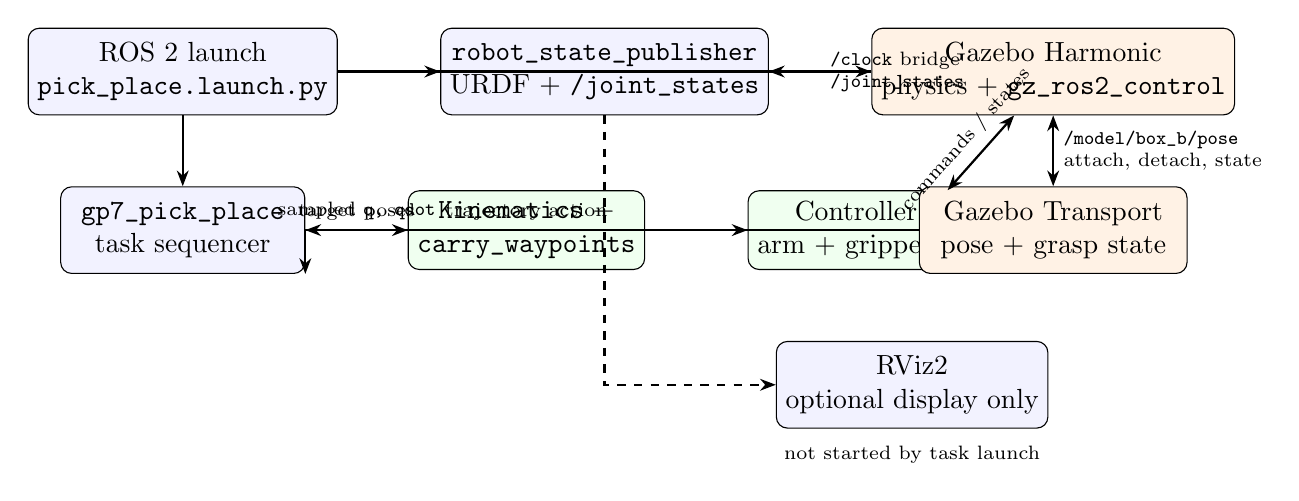
\begin{tikzpicture}[
  node distance=9mm and 13mm,
  block/.style={draw,rounded corners,align=center,minimum width=31mm,minimum height=11mm,fill=blue!5},
  data/.style={draw,rounded corners,align=center,minimum width=28mm,minimum height=10mm,fill=green!6},
  gz/.style={draw,rounded corners,align=center,minimum width=34mm,minimum height=11mm,fill=orange!10},
  link/.style={-{Stealth[length=2mm]},thick},
  bidir/.style={{Stealth[length=2mm]}-{Stealth[length=2mm]},thick}
]
\node[block] (launch) {ROS 2 launch\\\code{pick_place.launch.py}};
\node[block,right=of launch] (rsp) {\code{robot_state_publisher}\\URDF + \code{/joint_states}};
\node[gz,right=of rsp] (gzsim) {Gazebo Harmonic\\physics + \code{gz_ros2_control}};
\node[block,below=of launch] (task) {\code{gp7_pick_place}\\task sequencer};
\node[data,right=of task] (motion) {\code{Kinematics} +\\\code{carry_waypoints}};
\node[data,right=of motion] (controllers) {Controller manager\\arm + gripper controllers};
\node[gz,below=of gzsim] (gztransport) {Gazebo Transport\\pose + grasp state};
\node[block,below=of controllers] (rviz) {RViz2\\optional display only};

\draw[link] (launch) -- (rsp);
\draw[link] (launch) -- (gzsim);
\draw[link] (launch) -- (task);
\draw[link] (task) -- node[above,sloped,font=\scriptsize]{target poses} (motion);
\draw[link] (motion) -- node[above,sloped,font=\scriptsize]{sampled \code{q, qdot}} (task);
\draw[link] (task) -- node[above,font=\scriptsize]{trajectory action} (controllers);
\draw[bidir] (controllers) -- node[above,sloped,font=\scriptsize]{commands / states} (gzsim);
\draw[link] (gzsim) -- node[right,font=\scriptsize,align=left]{\code{/clock} bridge\\\code{/joint_states}} (rsp);
\draw[bidir] (gzsim) -- node[right,font=\scriptsize,align=left]{\code{/model/box_b/pose}\\attach, detach, state} (gztransport);
\draw[link] (gztransport.west) -| (task.south east);
\draw[link,dashed] (rsp.south) |- (rviz.west);
\node[font=\scriptsize,below=1mm of rviz] {not started by task launch};
\end{tikzpicture}
}
\caption{Actual task-side processes and data paths. The clock is explicitly
bridged; model pose and grasp feedback use Gazebo Transport in the task node.}
\label{fig:architecture}
\end{figure}

\section{Execution from launch command to placed object}
At launch, ROS resolves the installed package-share paths. The launch file
reads the configured mode and seed, computes or samples a Box B pickup, writes
that position into a temporary SDF world, reads the GP7 URDF, calls
\code{task_description}, and starts Gazebo with the generated world. The same
task URDF is sent to robot-state publisher and the Gazebo create node. The
launch starts the broadcaster, arm controller, and gripper controller;
\code{pick_place_node} is launched only when the spawner process exits
successfully and \code{run_task} is true.

The node waits for nonzero simulation clock, a complete arm \code{/joint_states}
message, Box B pose, and the arm action server. It asks for an initial detach
confirmation because the Gazebo plugin begins attached. It checks pickup pose
and upright orientation, computes the approach IK, and builds every Cartesian
segment before moving. It then opens, approaches, descends, checks grasp-frame
error, closes, attaches, transfers while monitoring feedback, checks
pre-release placement, detaches, opens, retreats, waits for settling, and
checks final translation and orientation before emitting success. Chapter 12
walks through each operation at code level.

\section{Input/output contracts}
The principal computational pipeline is
\begin{equation}
 (\text{URDF},\ \text{pickup},\ \text{destination})
 \longrightarrow \text{target Cartesian waypoints}
 \longrightarrow (t_k,\qvec_k,\dot{\qvec}_k)
 \longrightarrow \texttt{FollowJointTrajectory}
 \longrightarrow \text{joint / box / grasp feedback}.
\end{equation}
The trajectory does not bypass the controller manager; the task serializes
sampled arrays into ROS trajectory points and sends them through the action
interface. Gazebo Transport feedback closes the monitoring loop for the box
and detachable-joint state.

\chapter{URDF, Robot Modeling, and Coordinate Frames}
\label{ch:urdf}

\section{The source is URDF, not Xacro}
The runtime model is the plain XML file
\file{gp7_ros2/gp7_description/urdf/gp7.urdf}. Although the Gazebo package
manifest declares an Xacro dependency, no Xacro file is present and the task
launch does not invoke Xacro. Instead, Python parses and edits XML text before
passing the expanded description to Gazebo and robot-state publisher. This is
an important repository-specific distinction.

\section{Link and joint semantics}
A URDF \code{link} is a rigid body with optional visual geometry, collision
geometry, and inertial properties. A URDF \code{joint} connects one parent
link to one child link. Its \code{origin} is the pose of the joint frame
relative to the parent link; its \code{axis} is expressed in the joint frame.
For a revolute joint, the scalar joint position rotates the child-side chain
about that axis. Fixed joints preserve a transform but add no degree of
freedom. The \code{Kinematics} parser follows parent/child links from
\code{base_link} to \code{grasp_frame}; at each joint it applies the fixed
origin and then the revolute rotation.

The authoritative chain includes the six arm revolute joints, a fixed flange,
fixed tool0, fixed gripper base, one driver and five mimic finger joints, and a
fixed grasp frame. The extra \code{base} link is fixed to \code{base_link} at
z=\SI{0.33}{m}; it is not another actuated joint. The world-to-base transform
is identity.

\section{Visual, collision, and inertial models}
Each GP7 arm link references separate visual and collision STL files. The
visual files preserve appearance; collision geometry determines contact and
may be lower detail. The seven adaptive gripper DAE files are referenced for
visuals and, in this URDF, the same DAE path also appears in collision tags.
The working URDF uses scale 1.5 for the gripper meshes while leaving arm
meshes at scale 1; this is a project model adaptation. The environment includes
a 20 m square plane. Box A is a
static collision/visual box of size $(0.30,0.30,0.20)$ m. Box B is a dynamic
$(0.05)^3$ m cube with mass \SI{0.05}{kg}.

The URDF gives every modeled robot link a mass of \SI{1}{kg} and diagonal
inertia entries of $0.01$ with zero products of inertia. These are repeated
placeholder-like values, not validated CAD mass properties. They can permit
simulation but should not be presented as an identified physical inertia
model. Box B has diagonal inertia entries $2.08333\times10^{-5}$ kg m$^2$,
consistent with a uniform cube using its stated mass and dimensions. Box A is
static and does not need a dynamic inertial model for this task.

\section{TF tree and time-varying transforms}
\code{robot_state_publisher} consumes the URDF and joint-state messages and
publishes transforms for the link tree. Fixed joint transforms do not change;
the six arm and active gripper joint transforms depend on current joint
positions. In a conventional TF tree, each child has one parent, matching the
URDF chain. Gazebo's object model pose is not automatically the same stream as
the robot's TF transform: this task separately subscribes to the Gazebo
Transport pose vector for \code{box_b}.

The fixed identity transform from \code{world} to \code{base_link} aligns
the planning base with the simulation world. This is why the world-coordinate
Box A target can be passed to the URDF-based FK/IK without an additional
world/base calibration transform. That assumption would have to be changed if
the robot were spawned at a nonidentity pose.

\section{Actual zero-pose DH geometry}
The DH frames are deliberately not identified with all URDF link frames. At
zero joint angles, the documented frame origins in base coordinates are
\begin{align*}
 o_0&=(0,0,0), &o_1&=(0.040,0,0.330),\\
 o_2&=(0.040,0,0.775), &o_3&=(0.040,0,0.815),\\
 o_4&=o_5=o_6=(0.480,0,0.815)\quad\text{(m)}.
\end{align*}
Frame 3 lies at the intersection of the extended elbow axis and wrist axes,
not at the URDF \code{link_4_r} origin. The coincident wrist-frame origins
reflect intersecting wrist axes. The terminal DH frame 6 is still distinct
from the tool0/grasp frame.

\begin{figure}[htbp]
\centering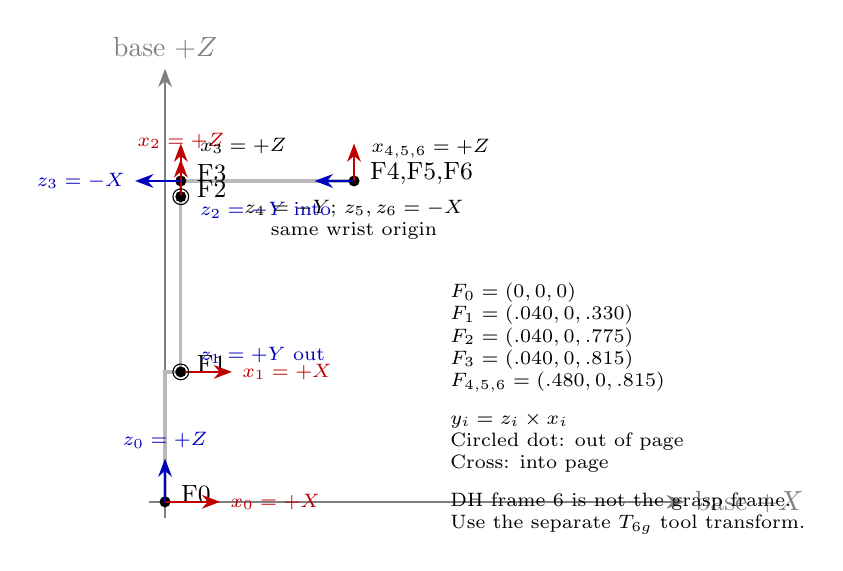
\begin{tikzpicture}[scale=1.0,>=Stealth]
  \draw[->,gray,thick] (-.2,0)--(6.6,0) node[right]{base $+X$};
  \draw[->,gray,thick] (0,-.2)--(0,5.5) node[above]{base $+Z$};
  % Origins projected into X-Z; y=0 at the zero configuration.
  \draw[very thick,gray!55] (0,0)--(0,1.65)--(.2,1.65)--(.2,3.875)--(.2,4.075)--(2.4,4.075);
  \foreach \x/\z/\lab in {0/0/F0,.2/1.65/F1,.2/3.875/F2,.2/4.075/F3,2.4/4.075/{F4,F5,F6}} {
    \fill (\x,\z) circle (2pt);
    \node[anchor=west,font=\small] at (\x+.08,\z+.10) {\lab};
  }
  % Frame 0 and 1 axes projected in plane.
  \draw[->,red!75!black,thick] (0,0)--(.7,0) node[right,font=\scriptsize]{$x_0=+X$};
  \draw[->,blue!75!black,thick] (0,0)--(0,.55) node[above,font=\scriptsize]{$z_0=+Z$};
  \draw[->,red!75!black,thick] (.2,1.65)--(.85,1.65) node[right,font=\scriptsize]{$x_1=+X$};
  \draw ( .2,1.65) circle (0.10); \fill (.2,1.65) circle (1.5pt);
  \node[anchor=west,font=\scriptsize,blue!75!black] at (.32,1.86){$z_1=+Y$ out};
  % F2 has z into page; x2 is vertical.
  \draw[->,red!75!black,thick] (.2,3.875)--(.2,4.35) node[above,font=\scriptsize]{$x_2=+Z$};
  \draw (.2,3.875) circle (.10); \draw (.15,3.825)--(.25,3.925); \draw (.15,3.925)--(.25,3.825);
  \node[anchor=west,font=\scriptsize,blue!75!black] at (.32,3.70){$z_2=-Y$ into};
  % Frame 3 x3=+Z, z3=-X.
  \draw[->,red!75!black,thick] (.2,4.075)--(.2,4.55);
  \draw[->,blue!75!black,thick] (.2,4.075)--(-.38,4.075) node[left,font=\scriptsize]{$z_3=-X$};
  \node[anchor=west,font=\scriptsize] at (.32,4.52){$x_3=+Z$};
  % Wrist center: axes differ in 3D while origin coincides.
  \draw[->,red!75!black,thick] (2.4,4.075)--(2.4,4.55);
  \draw[->,blue!75!black,thick] (2.4,4.075)--(1.9,4.075);
  \node[anchor=west,font=\scriptsize] at (2.5,4.48){$x_{4,5,6}=+Z$};
  \node[anchor=north,font=\scriptsize,align=center] at (2.4,3.96){$z_4=-Y$; $z_5,z_6=-X$\\same wrist origin};
  \node[anchor=north west,font=\scriptsize,align=left] at (3.5,2.9){
    $F_0=(0,0,0)$\\
    $F_1=(.040,0,.330)$\\
    $F_2=(.040,0,.775)$\\
    $F_3=(.040,0,.815)$\\
    $F_{4,5,6}=(.480,0,.815)$\\[2mm]
    $y_i=z_i\times x_i$\\
    Circled dot: out of page\\
    Cross: into page\\[2mm]
    DH frame 6 is not the grasp frame.\\
    Use the separate $T_{6g}$ tool transform.
  };
\end{tikzpicture}

\caption{Standard-DH origin schematic projected into base X--Z. All pictured
origins lie at $y=0$ at home. Out-of-plane axis signs and origin coordinates
are annotated. The diagram is a kinematic construction, not a mesh rendering.}
\label{fig:dh-frames}
\end{figure}

\section{URDF fixed transforms near the tool}
Three fixed transforms matter in the DH-to-runtime comparison:
\begin{enumerate}
 \item \code{joint_6_t-flange}: $p=(0.080,0,0)$ m, zero RPY.
 \item \code{flange-tool0}: $p=(0,0,0)$ and RPY
 $(3.14159265,-1.57079632,0)$ rad.
 \item \code{tool0_to_grasp_frame}: $p=(-0.0009111,0.0123,0.14598)$ m,
 zero RPY.
\end{enumerate}
Replacing the decimal RPY angles by exact $\pi$ values is a convenient
derivation approximation but slightly changes the transform. The verification
script reads the exact URDF values.

\section{ros2\_control model embedded in URDF}
The URDF's \code{ros2_control} element declares a \code{GazeboSystem} with
\code{gz_ros2_control/GazeboSimSystem}. Each arm joint and the gripper
driver has a position command interface and position/velocity state
interfaces. The five mimic joints expose state interfaces but no command
interfaces. The external plugin loads the controller manager inside the
simulator and connects these abstract interfaces to Gazebo joint state and
command components. The project YAML chooses the actual controller instances.

\section{CAD exports versus runtime model}
The repository contains at least two CAD-exported GP7 URDFs in addition to the
runtime file: \file{GP7 (Solidworks 2020)/GP7 components/GP7/GP7.urdf} and
\file{GP7 (Solidworks 2020)/URDF/Build/Build.urdf}. They have distinct tree,
path, and mesh context and are not silently interchangeable. The task launch,
DH verification, and regression tests all target
\file{gp7_ros2/gp7_description/urdf/gp7.urdf}. A separate CAD-fidelity study
would need to compare origins, scaling, joint axes, and mesh coordinate frames
before claiming equivalence.

\chapter{Standard Denavit--Hartenberg Parameters}
\label{ch:dh}

\section{Convention and geometry}
The project derives its table using \textbf{standard DH}:
\begin{equation}
 A_i=R_z(\theta_i)\,T_z(d_i)\,T_x(a_i)\,R_x(\alpha_i),
 \qquad {}^{i-1}T_i=A_i.
 \label{eq:standard-dh-order}
\end{equation}
The revolute coordinate $\theta_i$ rotates about $z_{i-1}$. After this
rotation, the offset $d_i$ moves along that axis. The common-normal displacement
$a_i$ is along $x_i$; finally $\alpha_i$ rotates about that common-normal axis
to align the next joint axis. Because the transforms act right-to-left on a
point, the matrix product is written in the order in \cref{eq:standard-dh-order}.
This is not modified DH; swapping $T_x$ and $R_x$ or using the modified-DH
table would change the kinematics.

For parameters $(\theta,d,a,\alpha)$, the homogeneous transform is
\begin{equation}
 A(\theta,d,a,\alpha)=
 \begin{bmatrix}
 c_\theta&-s_\theta c_\alpha&s_\theta s_\alpha&a c_\theta\\
 s_\theta&c_\theta c_\alpha&-c_\theta s_\alpha&a s_\theta\\
 0&s_\alpha&c_\alpha&d\\0&0&0&1
 \end{bmatrix}.
 \label{eq:dh-general}
\end{equation}
The $\alpha$ and $d$ values are signed coordinate displacements and rotations;
they need not be positive physical link lengths. Frame axes must form
right-handed orthonormal triads, with $y_i=z_i\times x_i$.

\section{Mapping URDF axes to DH axes}
All six arm joint origins in the simulation URDF have zero RPY. Their joint
origin positions and local axes are in \cref{tab:arm-joints}. At the zero
configuration, the DH joint axes are chosen as
\begin{align}
 z_0&=+Z, &z_1&=+Y, &z_2&=-Y,\\
 z_3&=-X, &z_4&=-Y, &z_5&=-X.
\end{align}
These choices reproduce the positive directions in the URDF. The corresponding
local joint axes and URDF origins are listed in \cref{tab:arm-joints}. DH frames are
free to differ from link frames as long as each $A_i$ maps correctly; the
table's $q_i$ remain the URDF joint positions in the same order.

\section{Frame-by-frame construction}
\begin{enumerate}[label=\textbf{Joint \arabic*:},leftmargin=*]
 \item \textbf{Base rotation S.} $z_0=+Z$ is the base yaw axis. $z_1=+Y$ is
 the shoulder axis at $(0.040,0,0.330)$ m. Their axes are perpendicular and
 offset by the base/shoulder geometry. Choose $x_1=+X$, the common normal
 direction. The vertical displacement is $d_1=0.330$ m and the common-normal
 offset is $a_1=0.040$ m. The $-\pi/2$ twist aligns the next z-axis with
 $+Y$. The joint angle is $\theta_1=q_1$.

 \item \textbf{Shoulder L.} $z_1=+Y$ and $z_2=-Y$ are antiparallel axes.
 The upper-arm separation is $0.445$ m along home $+Z$, so choose
 $x_2=+Z$ and $a_2=0.445$ m. The antiparallel axis choice gives
 $\alpha_2=\pi$. The URDF zero shoulder angle must place $x_2$ along $+Z$;
 with the chosen preceding frame this requires the fixed offset
 $\theta_2=q_2-\pi/2$. There is no $d_2$ translation.

 \item \textbf{Elbow U.} $z_2=-Y$ and $z_3=-X$ define perpendicular axes.
 The short elbow offset is $0.040$ m along $+Z$ (the common normal), giving
 $a_3=0.040$ m. The chosen twist is $\alpha_3=-\pi/2$ and the angle is
 $\theta_3=q_3$. There is no z-offset.

 \item \textbf{Wrist roll R.} $z_3=-X$ and $z_4=-Y$ intersect at the wrist
 axis geometry after moving to the wrist center. The center is displaced
 $+0.440X$ from frame 3, opposite $z_3$; hence the signed parameter is
 $d_4=-0.440$ m. Since the axes intersect, $a_4=0$. The table uses
 $\alpha_4=+\pi/2$ and $\theta_4=q_4$.

 \item \textbf{Wrist bend B.} $z_4=-Y$ and $z_5=-X$ intersect at the same
 wrist center, so $a_5=d_5=0$. The selected twist is $\alpha_5=-\pi/2$ and
 the revolute coordinate is $\theta_5=q_5$.

 \item \textbf{Wrist twist T.} $z_5$ and $z_6$ are both $-X$ at the same
 point. There is no translation or twist, so $a_6=d_6=\alpha_6=0$, with
 $\theta_6=q_6$.
\end{enumerate}

The origin/axis picture is in \cref{fig:dh-frames}. It is a home-pose X--Z
projection; axes parallel to base $Y$ are marked out of or into the page.
The signed offset $d_4=-0.440$ is particularly easy to misread: the actual
hardware separation is positive length, but the selected $z_3$ coordinate
points opposite the displacement.

\section{Verified DH table}
\begin{table}[htbp]
\centering
\caption{Verified standard-DH parameters for the task URDF. Angles are in
radians, distances in metres.}
\label{tab:dh}
\begin{tabular}{c l r r r l}
\toprule $i$ & axis & $a_i$ & $\alpha_i$ & $d_i$ & $\theta_i$\\\midrule
1&S&0.040&$-\pi/2$&0.330&$q_1$\\
2&L&0.445&$\pi$&0&$q_2-\pi/2$\\
3&U&0.040&$-\pi/2$&0&$q_3$\\
4&R&0&$\pi/2$&-0.440&$q_4$\\
5&B&0&$-\pi/2$&0&$q_5$\\
6&T&0&0&0&$q_6$\\\bottomrule
\end{tabular}
\end{table}

Only the geometry columns $a_i,\alpha_i,d_i$ are constant. Each $q_i$ is
variable, and the sole constant angular correction is $-\pi/2$ in the second
row. The mapping preserves the URDF joint names and signs: there are no
additional sign inversions.

\section{Derivation of all six matrices}
Define $c_i=\cos q_i$, $s_i=\sin q_i$, and
$v_2=q_2-\pi/2$. Substitution into \cref{eq:dh-general} yields
\begin{align}
A_1&=\begin{bmatrix}
c_1&0&-s_1&0.040c_1\\s_1&0&c_1&0.040s_1\\0&-1&0&0.330\\0&0&0&1
\end{bmatrix},\\[1mm]
A_2&=\begin{bmatrix}
\cos v_2&\sin v_2&0&0.445\cos v_2\\
\sin v_2&-\cos v_2&0&0.445\sin v_2\\
0&0&-1&0\\0&0&0&1
\end{bmatrix},\\[1mm]
A_3&=\begin{bmatrix}
c_3&0&-s_3&0.040c_3\\s_3&0&c_3&0.040s_3\\0&-1&0&0\\0&0&0&1
\end{bmatrix},\\[1mm]
A_4&=\begin{bmatrix}
c_4&0&s_4&0\\s_4&0&-c_4&0\\0&1&0&-0.440\\0&0&0&1
\end{bmatrix},\\[1mm]
A_5&=\begin{bmatrix}
c_5&0&-s_5&0\\s_5&0&c_5&0\\0&-1&0&0\\0&0&0&1
\end{bmatrix},\\[1mm]
A_6&=\begin{bmatrix}
c_6&-s_6&0&0\\s_6&c_6&0&0\\0&0&1&0\\0&0&0&1
\end{bmatrix}.
\label{eq:all-dh-matrices}
\end{align}
For example, row 1 has $\alpha_1=-\pi/2$, so
$\cos\alpha_1=0$ and $\sin\alpha_1=-1$. Inserting those into the general
matrix gives its second and third columns and confirms the negative sign in
the $(3,2)$ entry. Row 2 uses $\cos\pi=-1$, which explains its negative
$\cos v_2$ entry. This substitution process is the safest way to catch common
DH sign errors.

\section{Base and tool transforms}
The world-to-base and base-to-DH-frame-0 transforms are identities in this
spawn configuration. Link \code{link_6_t} to the selected DH frame 6 has
rotation
\begin{equation}
 C=\begin{bmatrix}0&0&-1&0\\0&1&0&0\\1&0&0&0\\0&0&0&1\end{bmatrix}.
\end{equation}
The fixed transform from frame 6 to grasp frame is constructed from the exact
URDF fixed joints:
\begin{equation}
 {}^6T_g=C^{-1}T_{link6,flange}T_{flange,tool0}T_{tool0,g}.
 \label{eq:dh-tool-transform}
\end{equation}
Numerically, using rounded values for display,
\begin{equation}
 {}^6T_g\approx\begin{bmatrix}
 1&0&0&-0.0009111\\0&-1&0&-0.0123\\0&0&-1&-0.22598\\0&0&0&1
 \end{bmatrix}.
\end{equation}
Then the chain actually compared against runtime FK is
\begin{equation}
 {}^BT_g(q)=A_1A_2A_3A_4A_5A_6\,{}^6T_g.
 \label{eq:dh-chain}
\end{equation}

\section{Independent derivation versus executable code}
The runtime \code{Kinematics.fk} does \emph{not} evaluate the six hard-coded
DH matrices. It traverses the URDF chain and multiplies each joint origin by
the rotation about that joint's normalized axis. The standalone
\file{docs/verify_dh.py} separately defines the table and matrix in
\cref{eq:dh-general}, builds the fixed tool transform, and compares its result
to URDF FK. This separation is valuable: if both computations reused the same
table implementation, agreement would be a weaker check.

The verifier also checks the URDF joint origins, zero RPY, and local axes
against expected source geometry. The DH table was chosen to fit this exact
task URDF. It has not been proven to reproduce the manufacturer CAD or the
other URDF exports stored under the SolidWorks directory.

\chapter{Forward Kinematics}
\label{ch:fk}

\section{What FK answers}
Forward kinematics maps known joint coordinates to the tool's position and
orientation. Given $\qvec$, each joint contributes a rigid transform. For a
serial chain, transforms compose by matrix multiplication because the output
frame of one joint becomes the input frame of the next. The result belongs to
$\SE(3)$ and has a rotation matrix and translation vector:
\begin{equation}
 {}^BT_g(\qvec)=
 \begin{bmatrix}{}^BR_g(\qvec)&{}^B\pvec_g(\qvec)\\0&1\end{bmatrix}.
 \label{eq:fk-result}
\end{equation}
The first three columns of the 3-by-3 block are the grasp frame's local unit
axes expressed in base coordinates. The last column is the grasp-frame origin
in metres.

\section{Transform-chain multiplication}
Under the standard-DH construction, FK is \cref{eq:dh-chain}:
\begin{equation}
 {}^BT_g=A_1A_2A_3A_4A_5A_6{}^6T_g.
\end{equation}
One can build intermediate poses
\begin{equation}
 {}^BT_1=A_1,\quad {}^BT_2=A_1A_2,\quad
 {}^BT_3=A_1A_2A_3,\quad {}^BT_6=A_1\cdots A_6,
\end{equation}
then apply the fixed tool transform to obtain ${}^BT_g$. In code, matrix
composition is associative but not commutative: swapping adjacent transforms
changes the reference frame and the physical result.

\section{Fully worked home example}
At $q_i=0$, $v_2=-\pi/2$. The individual matrices reduce to
\begin{align*}
A_1&=\begin{bmatrix}1&0&0&.040\\0&0&1&0\\0&-1&0&.330\\0&0&0&1\end{bmatrix},&
A_2&=\begin{bmatrix}0&-1&0&0\\-1&0&0&-.445\\0&0&-1&0\\0&0&0&1\end{bmatrix},\\
A_3&=\begin{bmatrix}1&0&0&.040\\0&0&1&0\\0&-1&0&0\\0&0&0&1\end{bmatrix},&
A_4&=\begin{bmatrix}1&0&0&0\\0&0&-1&0\\0&1&0&-.440\\0&0&0&1\end{bmatrix},\\
A_5&=\begin{bmatrix}1&0&0&0\\0&0&1&0\\0&-1&0&0\\0&0&0&1\end{bmatrix},&A_6&=I_4.
\end{align*}
Multiplying the first six produces the DH wrist-frame origin $(0.480,0,0.815)$
m and orientation $C_{3\times3}$. Applying ${}^6T_g$ moves the grasp point
approximately $(+0.225980,-0.012300,-0.000911)$ m in base coordinates. Thus
\begin{equation}
 {}^BT_g(0)\approx
 \begin{bmatrix}
 0&0&1&0.705980\\
 0&-1&0&-0.012300\\
 1&0&0&0.814089\\
 0&0&0&1
 \end{bmatrix}.
 \label{eq:home-fk}
\end{equation}
The tiny off-axis entries in direct floating-point URDF evaluation are caused
by the URDF's decimal approximations to $\pi$; \cref{eq:home-fk} is rounded.

\section{Worked nonzero configuration}
The independently recorded verification example
$\qvec=(0.4,0.6,1.2,-0.7,0.8,1.1)$ rad lies within the six arm joint limits.
Applying the URDF chain gives the following rounded pose:
\begin{equation}
{}^BT_g\approx\begin{bmatrix}
-0.857809731&-0.290135590&0.424244982&0.675035771\\
0.156339523&-0.933613380&-0.322372473&0.161569746\\
0.489612519&-0.210207986&0.846222302&1.166928133\\
0&0&0&1
\end{bmatrix}.
\label{eq:fk-nonzero-example}
\end{equation}
The position result is therefore approximately
$(0.675036,0.161570,1.166928)$ m. The rotation's column vectors remain unit
length and mutually orthogonal up to round-off, and its determinant is one.
This is a mathematical FK example, not a measured Gazebo pose.

\section{Executable URDF FK}
\code{gp7_motion/kinematics.py} parses the URDF into a list of transforms and
axes in \code{Kinematics.__init__}. For each chain joint,
\code{fk(q)} first right-multiplies the static joint origin. If the joint is
revolute, it then right-multiplies a rotation generated from the normalized
axis multiplied by its corresponding $q_i$. Fixed joints contribute only
their static transform. Because the chain starts at \code{base_link} and
ends at \code{grasp_frame}, the return value is already the base-to-grasp
transform.

No arm dimensions are duplicated in the runtime FK or IK: changing the URDF
joint origin updates these computations. This reduces parameter drift between
the model and planner, though it means a malformed URDF can also corrupt both
the runtime results and any tests that reuse the same parser.

\section{Independent DH agreement check}
\file{docs/verify_dh.py} independently builds DH matrices using a separately
stated table and reads the exact URDF fixed tool transforms. It checks four
explicit configurations, then 100 deterministic joint vectors drawn uniformly
between the parsed lower and upper limits using NumPy generator seed 42. It
compares translation by Euclidean norm and rotation by the angle of the
relative rotation. In the verification recorded on 14 November 2026, all 104
passed with maximum errors
\begin{equation}
 \max_k\|p_{DH,k}-p_{URDF,k}\|_2=5.50\times10^{-16}\si{m},\qquad
 \max_k\angle(R_{DH,k}^{T}R_{URDF,k})=4.93\times10^{-16}\si{rad}.
\end{equation}
These are machine-precision comparisons of two calculations for the same
implemented URDF. They do not measure physical robot accuracy or CAD fidelity.

\section{Reproduce the FK check}
From the repository root after installing system NumPy/SciPy, use:
\begin{lstlisting}[language=bash]
/usr/bin/python3 docs/verify_dh.py
\end{lstlisting}
The script is read-only. Its current recorded output prints each explicit
configuration's errors and the maximum over all 104. Chapter 13 distinguishes
this mathematical check from the dynamic Gazebo run.

\chapter{Inverse Kinematics}
\label{ch:ik}

\section{From desired pose to joint coordinates}
Inverse kinematics reverses FK. Given a desired grasp position $p_d$ and
orientation $R_d$, find a joint vector $\qvec$ for which
\begin{equation}
 {}^BT_g(\qvec)\approx
 \begin{bmatrix}R_d&p_d\\0&1\end{bmatrix}.
\end{equation}
There may be multiple joint configurations with the same tool pose; some
targets have no solution inside the robot's workspace or joint limits, and
near singular configurations the required joint changes can become very
large. IK is consequently a constrained search, not simply inverting a square
matrix.

\section{The method actually implemented}
The runtime calls SciPy's bounded nonlinear least-squares routine
\code{scipy.optimize.least_squares}. For candidate $q$, it computes the
URDF-based pose and forms a six-element residual:
\begin{equation}
 r(\qvec)=
 \begin{bmatrix}
 p_{FK}(\qvec)-p_d\\
 \mathrm{rotvec}(R_d^TR_{FK}(\qvec))
 \end{bmatrix}\in\R^6.
 \label{eq:ik-residual}
\end{equation}
The first three terms are position error in metres. The last three terms are
the rotation vector (axis times angle) of the relative rotation, in radians.
The implementation concatenates these quantities without scaling or a
separate translation/rotation weighting. Consequently the norm threshold is
a numerical code criterion, not a dimensionally homogeneous physical metric.

The solver bounds are read from URDF limits. Before each solve, the initial
guess is clipped to lie $10^{-8}$ inside each bound, avoiding an initial
coordinate exactly on a boundary. The solve uses at most 150 function
evaluations and sets \code{ftol=xtol=gtol=1e-10}. It accepts a result only if
$\|r(q)\|_2<10^{-6}$; otherwise it tries another seed or raises
\code{ValueError}. The implementation does not provide a custom analytic
Jacobian, collision constraints, posture cost, or task-space damping policy.
SciPy's solver handles its internal local model and numerical derivative
behavior according to the installed SciPy defaults.

\section{Initialization and branch continuity}
For a normal Cartesian sample, the seed is the previous sample's returned
joint vector. This encourages a nearby solution branch and avoids restarting
from a home posture at every millisecond-scale waypoint. The code also rejects
a segment if the maximum adjacent joint step exceeds $0.15$ rad. This is a
discontinuity guard, not a proof that the branch is globally optimal.

When \code{restart=True}, the first guess is followed by 24 additional vectors
sampled uniformly within the URDF limits using a deterministic NumPy random
generator seeded to 7. The task uses restarts for its initial above-pickup
approach IK; each later Cartesian sample is warm-started from its predecessor
without random restarts. Multiple restart attempts improve the chance of
finding a feasible branch but do not enumerate every IK solution.

\section{Worked solver example}
During this guide's source-based numerical check, the runtime solver was asked
for a downward-oriented grasp at
\begin{equation}
 p_d=(0.55,0.35,0.40)\si{m},\qquad R_d=\mathrm{diag}(1,-1,-1),
\end{equation}
with zero seed and deterministic restarts. One returned solution was
\begin{equation}
 \qvec\approx(0.58172582,\ 0.44238155,\ 0.10901428,\ 0,\ -1.23742905,\ -0.58172582)^T\si{rad}.
 \label{eq:ik-example}
\end{equation}
Substituting this vector back into runtime FK gave
$p_{FK}=(0.55,0.35,0.40)$ m to displayed precision and orientation error
$1.9\times10^{-16}$ rad. It is one numerical solution for this solver/version,
not a unique closed-form answer and not a Gazebo task result. A different
valid initial seed may select another joint configuration.

\section{Singularities, unreachable poses, and limits}
A singularity occurs when small tool motion cannot be produced by an ordinary
small change in all independent task directions, or when the inverse mapping
becomes ill-conditioned. The far-pickup optimizer identifies the straight
elbow as its exact horizontal boundary. The selected point is moved inward by
\SI{5}{mm} before route planning to leave margin for tracking and continuous
IK. This is a model-specific constrained, downward-tool envelope, not the
maximum radius for every orientation.

Joint bounds are part of the least-squares problem. A target at $(5,5,5)$ m is
explicitly expected to fail and is covered by an offline test. Other
infeasible goals can fail from nonconvergence even when a simple geometric
reach bound does not rule them out. The segment planner then aborts before
physical motion because the task constructs all route segments before sending
the approach trajectory.

\section{What is not implemented}
The model has a six-axis wrist geometry often associated with closed-form
solutions, but the code does not algebraically solve shoulder/elbow/wrist
branches. It does not build or expose an arm Jacobian, use a pseudoinverse
update $q_{k+1}=q_k+J^+e$, optimize a nullspace objective, or perform
collision-aware IK. Such equations are useful theory, but must not be
presented as this project's method. The actual solver is the residual-based,
bounded nonlinear least-squares procedure described above.

\section{Connection to command generation}
IK returns one $q$ for each Cartesian interpolation sample. The trajectory
code places those joint vectors and estimated velocities into a sequence of
\code{JointTrajectoryPoint} messages. The task node sends the sequence through
the \code{FollowJointTrajectory} action and checks both the action result and
measured joint positions when it completes. Thus successful IK alone does not
move the robot; it produces reference states for the ROS 2 controller.

\chapter{Trajectory Planning}
\label{ch:trajectory}

\section{Joint-space and Cartesian-space paths}
A path specifies the geometric states to visit; a time law specifies how fast
to traverse them. Joint-space planning directly interpolates the six
coordinates $q_i$. Cartesian planning specifies a straight-line tool-position
segment and a fixed tool orientation, then solves IK at each sampled point.
The project uses both: the initial approach uses a joint-space quintic
segment, while descent/lift/transfer/lower/retreat use Cartesian segments.

The Cartesian tool orientation is fixed to
\begin{equation}
 R_{down}=\mathrm{diag}(1,-1,-1),\qquad \det(R_{down})=+1,
\end{equation}
which is a 180-degree rotation about base/tool x: tool $+x$ stays $+X$, while
tool $+y$ and $+z$ reverse. The matrix is a proper rotation and points the
grasp direction downward under this tool convention.

\section{Quintic time scaling}
For normalized time $u=t/T\in[0,1]$, the implemented blend is
\begin{equation}
 s(u)=10u^3-15u^4+6u^5.
 \label{eq:quintic}
\end{equation}
Its derivatives are
\begin{align}
 s'(u)&=30u^2-60u^3+30u^4,\\
 s''(u)&=60u-180u^2+120u^3.
\end{align}
At $u=0$ and $u=1$, $s$ reaches its endpoint values while $s'$ and $s''$ are
zero. This gives a rest-to-rest scalar interpolation with zero endpoint
velocity and acceleration for a linearly parameterized coordinate. The
dimensionless derivatives are scaled by $1/T$ and $1/T^2$ for physical
velocity and acceleration.

\begin{figure}[htbp]
\centering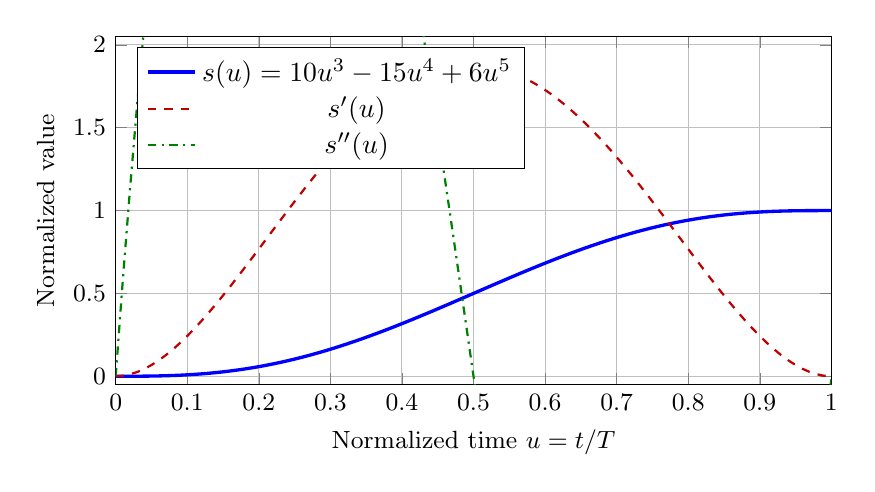
\begin{tikzpicture}
\begin{axis}[
  width=.88\textwidth,height=6cm,
  xlabel={Normalized time $u=t/T$},ylabel={Normalized value},
  xmin=0,xmax=1,ymin=-.05,ymax=2.05,
  grid=both,legend pos=north west,
  tick label style={font=\small},label style={font=\small},
  domain=0:1,samples=100
]
\addplot[blue,very thick] {10*x^3-15*x^4+6*x^5};
\addlegendentry{$s(u)=10u^3-15u^4+6u^5$}
\addplot[red!75!black,thick,dashed] {30*x^2-60*x^3+30*x^4};
\addlegendentry{$s'(u)$}
\addplot[green!50!black,thick,dashdotted] {60*x-180*x^2+120*x^3};
\addlegendentry{$s''(u)$}
\end{axis}
\end{tikzpicture}

\caption{Position blend and its derivatives for the quintic scalar time law.
This is the intended analytical profile, not a measured joint trace.}
\label{fig:quintic}
\end{figure}

For a joint-space segment, the code applies this blend directly:
\begin{equation}
 q(t)=q_0+s(t/T)(q_f-q_0),\quad
 \dot q(t)=\frac{s'(t/T)}{T}(q_f-q_0).
 \label{eq:joint-quintic}
\end{equation}
It samples at approximately \SI{50}{ms} intervals. The base duration defaults
to 8 s for the approach, then time-stretches if a sampled speed exceeds the
allowed joint speed cap.

\section{Cartesian segment construction}
For a Cartesian segment from $p_0$ to $p_f$, the implementation evaluates
\begin{equation}
 p(u)=p_0+s(u)(p_f-p_0),\qquad R(u)=R_{down}.
\end{equation}
It generates samples with nominal interval no greater than \SI{50}{ms}, solves
IK sequentially using the preceding $q$ as the next seed, and stores each
joint solution. The segment refuses to start unless its current tool
orientation is within $10^{-4}$ rad of the downward target. It refuses a
joint branch with adjacent sampled joint displacement above 0.15 rad.

Because the mapping $p\mapsto q$ is nonlinear, the resulting $q_i(t)$ values
do not each follow the scalar quintic equation exactly. The implementation
estimates joint velocity using \code{numpy.gradient} over sampled IK points,
then forces the first and last velocity vectors to zero. Unlike the joint
segment, it does not compute the analytic second derivative of the IK path.
The theoretical zero endpoint Cartesian acceleration should therefore not be
reported as a measured joint-acceleration guarantee.

\section{Velocity cap and duration stretching}
The allowed speed per joint is
\begin{equation}
 v_{cap,i}=\min(v_{URDF,i},0.5\si{rad/s}).
\end{equation}
For sampled joint speed estimates, the time scale is
\begin{equation}
 \lambda=\max\left(1,\max_{k,i}\frac{|\dot q_{k,i}|}{v_{cap,i}}\right).
 \label{eq:time-stretch}
\end{equation}
The code multiplies all timestamps by $\lambda$ and divides the sampled
velocities by $\lambda$. It samples and checks velocity; it does not impose a
measured acceleration or jerk limit. This is reference-trajectory scaling,
not feedback torque/velocity control. The Gazebo controller's position
command interface tracks the supplied trajectory.

\section{Scene-specific waypoint schedule}
The far route avoids a diagonal sweep through the base. It first descends to
the pickup (5 s), lifts to $z=0.10$ m (5 s), moves inward and gains height
through $(0.45,-0.45,0.40)$ m (7 s), transfers above Box A at $z=0.40$ m (6 s),
lowers to $z=0.226$ m (4 s), and retreats to the overhead target (4 s). The
initial approach to the above-pickup posture has nominal duration 8 s. Near
pickup instead lifts directly to $z=0.40$ m before transfer. These durations
are nominal; time scaling can extend them. They are hand-designed for this
scene and are not generated by collision search.

\section{Controller sampling and what is actually smooth}
The planned arrays are serialized into trajectory points with position,
velocity, and relative time. The arm controller exposes a position command
interface and position/velocity state interfaces. The quintic curve is smooth
within each generated segment at the scalar level, but the project does not
record per-joint traces, compute inter-segment acceleration discontinuity, or
validate jerk. The offline test resamples joint trajectories with a cubic
Hermite spline and checks sampled bounds, speed, endpoint, and orientation; it
does not prove Gazebo's exact interpolation or physical drive behavior.

\chapter{ROS 2 Controllers and Communication}
\label{ch:ros2}

\section{Nodes, graph, and interfaces}
ROS 2 nodes are independent processes or components connected by typed
interfaces. Topics stream state/events, services perform request-response
operations, and actions represent longer tasks with acceptance, feedback,
completion, and cancellation. The project uses all three general styles in
its ecosystem: topics for joint/gripper/stop streams, the
\code{FollowJointTrajectory} action for arm motion, and controller-manager
services for inspection. In the task path, the detachable-joint endpoints are
Gazebo Transport topics, not ROS services. ROS 2's own guide explains the
topic/service/action distinction \cite{ros2_interfaces}.

\section{Controller manager and hardware interfaces}
The URDF instantiates the external Gazebo simulated hardware system. The YAML
sets controller-manager update rate to \SI{100}{Hz} and simulation time. It
loads:
\begin{enumerate}
 \item \code{joint_state_broadcaster/JointStateBroadcaster};
 \item \code{joint_trajectory_controller/JointTrajectoryController} for
 all six arm joints;
 \item \code{position_controllers/JointGroupPositionController} for the
 single \code{gripper_driver} joint.
\end{enumerate}
The arm controller claims a \code{position} command interface and reads
\code{position} and \code{velocity} state interfaces. The gripper position
controller receives an array with one driver position. The five mimic joints
have state interfaces but no direct command interface in the URDF.

The joint trajectory controller exposes an action endpoint
\begin{center}\code{/arm_controller/follow_joint_trajectory}\end{center}
using \code{control_msgs/action/FollowJointTrajectory}. The project sends a
joint-name list and time-stamped \code{JointTrajectoryPoint} values with
positions and velocities. It checks acceptance, terminal status, action error
code, then compares final joint feedback with the final commanded point.
Controller package documentation is cited for interface semantics, while the
project YAML/code is authoritative for what is configured here
\cite{ros2_control_jtc}.

\section{ROS topics and message types}
\begin{longtable}{p{.39\textwidth}p{.26\textwidth}p{.29\textwidth}}
\caption{Important ROS interfaces visible in project source.}\label{tab:ros-interfaces}\\
\toprule Name & Type & Actual use\\\midrule\endfirsthead
\toprule Name & Type & Actual use\\\midrule\endhead
\code{/joint_states} & \code{sensor_msgs/msg/JointState} & Broadcaster feedback; task and manual arm node read arm positions; task also reads gripper driver angle.\\
\code{/arm_controller/follow_joint_trajectory} & \code{control_msgs/action/FollowJointTrajectory} & Task and manual arm/demo nodes send multi-point arm goals.\\
\code{/gripper_controller/commands} & \code{std_msgs/msg/Float64MultiArray} & Task and manual gripper node publish the single driver setpoint.\\
\code{/gp7/stop} & \code{std_msgs/msg/Empty} & Task node requests cancellation; manual arm node also handles stop. Not a safety-rated emergency stop.\\
\code{/gp7/goal_index} & \code{std_msgs/msg/Int32} & Manual arm preset selector (0--3), not used by assignment task node.\\
\code{/gp7/gripper_cmd} & \code{std_msgs/msg/Float64} & Manual gripper-node input, translated into controller command array.\\
\code{/clock} & \code{rosgraph_msgs/msg/Clock} & Gazebo clock bridged to ROS; nodes use simulation time.\\
\code{/controller_manager/list_controllers} & ListControllers service & Human-operated controller readiness check documented in README; task launch spawners wait for startup.\\
\bottomrule
\end{longtable}

The exact action and topic names are absolute names in the source. Controller
names in the YAML are \code{joint_state_broadcaster}, \code{arm_controller},
and \code{gripper_controller}. The Gazebo system creates the controller
manager. Both Gazebo launch descriptions enforce broadcaster startup before
or alongside the command controllers; the generic launch has a process-exit
event handler that starts arm and gripper spawners only after the broadcaster
spawner finishes.

\section{Gazebo Transport interfaces used alongside ROS}
These endpoints are native Gazebo Transport messages, despite their topic-like
names. The task code imports them from the vendor binding rather than through
\code{ros_gz_bridge}:
\begin{table}[htbp]
\centering\small
\caption{Gazebo Transport messages in \code{PickPlace}.}\label{tab:gz-interfaces}
\begin{tabularx}{\textwidth}{l l X}
\toprule Gazebo topic & Message type & Direction and purpose\\\midrule
\code{/gp7/grasp/attach} & \code{gz.msgs.Empty} & Task publishes; detachable-joint plugin attaches Box B.\\
\code{/gp7/grasp/detach} & \code{gz.msgs.Empty} & Task publishes; plugin removes attachment.\\
\code{/gp7/grasp/state} & \code{gz.msgs.StringMsg} & Plugin publishes text state such as \code{attached} / \code{detached}; task subscribes.\\
\code{/model/box_b/pose} & \code{gz.msgs.Pose_V} & SDF pose-publisher system sends model pose vector; task subscribes and selects the \code{box_b} entry.\\
\bottomrule
\end{tabularx}
\end{table}
The launch does not bridge these four topics into ROS. Only the simulation
clock has the explicit ROS--Gazebo bridge in the task launch. This split is
why a ROS topic listing alone does not show every interface used in the task.

\section{Robot-state publisher and TF}
\code{robot_state_publisher} receives the robot description and joint
states. It publishes fixed transforms for fixed URDF joints and dynamic
transforms for actuated joints. The task launch sets \code{use_sim_time}
and creates a \code{ros_gz_bridge} parameter bridge for \code{/clock}.
RViz in the separate display launch reads these transforms to render the URDF.
The assignment task itself does not rely on an RViz node.

\section{Manual control nodes versus the task node}
\code{ArmControllerNode} in \file{scripts/arm_controller_node.py} listens
for one of four preset indices, subscribes to joint states, and sends action
goals. Its stop callback cancels the active action and attempts a hold using
the last observed joint position. \code{GripperControllerNode} accepts a
simple scalar, checks finite value and $[-0.5,0.15]$ bounds, and publishes a
one-element array. \code{DemoSequenceNode} runs scripted joint waypoints and
gripper commands. These are separate manual/demo utilities; none performs
the integrated feedback-checked Box A/Box B workflow.

The task node itself bypasses these two wrapper nodes: it publishes directly
to \code{/gripper_controller/commands}, sends the arm action directly, and
subscribes to \code{/gp7/stop}. This matters when tracing nodes in a graph:
the arm and gripper wrappers need not be running during \code{pick_place.launch.py}.

\section{Communication diagram}
\Cref{fig:architecture} shows launch, state publisher, controller manager,
Gazebo, and the task. The clock path is bridged from Gazebo Transport into
ROS. Conversely, \code{pick_place_node.py} creates its own
\code{gz.transport13.Node}; it directly advertises and subscribes to grasp
and model-pose topics. Therefore not every connection in the task is a ROS 2
topic, and topic names alone do not identify the middleware type.

\section{Command, feedback, and failure handling}
An action goal has a lifecycle: the controller can reject it; an accepted
goal can finish with a result code; or the task can request cancellation. The
task's \code{move} function waits for the goal response, stores the active
handle, waits with a duration-based timeout, cancels on exception, checks
success, waits for settling, and compares live joint feedback. During carrying,
it also checks that pose and grasp-state feedback remain fresh and that the
largest observed orientation error remains within one degree. This adds
application-level checking around the controller action.

\chapter{Gazebo Simulation and Gripper}
\label{ch:gazebo}

\section{World and physics}
\file{gp7_ros2/gp7_gazebo/worlds/pick_place.sdf} defines the
\code{gp7_pick_place} world. It loads physics, user commands, and scene
broadcasting systems; applies gravity $(0,0,-9.81)$ m/s$^2$; and configures a
nominal maximum physics step of \SI{0.001}{s} and real-time factor 1. The
selected physics engine was observed to warn that mimic constraints are not
supported. The environment includes a directional light and static ground
plane.

Box A is a static blue box of size $(0.30,0.30,0.20)$ m with its model center
at $(0.55,0.35,0.10)$ m. This corresponds to the ground-referenced position
$(0.55,0.35,0)$ m used in the documentation. Box B is a dynamic red cube of
side \SI{0.05}{m}, mass \SI{0.05}{kg}, and center height \SI{0.025}{m} when on
the ground. The world file starts it at $(0.55,-0.20,0.025)$ m; the task
launch creates a temporary edited world for either far or seeded-near pickup.
Gazebo's pose publisher emits model pose vectors at \SI{50}{Hz}.

\section{Robot spawn and control coupling}
The task launch calls the \code{ros_gz_sim create} executable with the
generated URDF string. The robot description contains the external
\code{gz_ros2_control/GazeboSimSystem} plugin and controller YAML path.
Gazebo then exposes simulated joint state/command interfaces to the ROS 2
controller manager. Controller actions and gripper command topics alter the
Gazebo robot. The clock bridge aligns ROS timers and task waits with simulated
time.

\section{Finger actuation and mimic limitation}
Only \code{gripper_driver} is commanded by the task. The URDF describes five
dependent finger revolute joints with mimic multipliers of $+1$ or $-1$. The
task's \code{fingers(target)} function interpolates from the observed current
driver angle to target using quintic scaling; its nominal duration is
\begin{equation}
 T_g=\max\left(1\si{s},\frac{|q_{target}-q_{start}|}{0.25\si{rad/s}}\right).
\end{equation}
It publishes at approximately \SI{20}{ms} simulation-time steps, waits an
additional \SI{0.4}{s}, and rejects if measured driver angle differs by more
than 0.02 rad. During task grasp the close target is $-0.162$ rad; the fully
open target is $+0.15$ rad. The manual wrapper allows commands down to
$-0.5$ rad, but the task does not use that full-close setting.

The physics engine warning means URDF mimic metadata did not establish
realistic finger coupling in the recorded simulation. A visually moving
driver or a successfully completing task is not evidence that both fingers
generated accurate, symmetric contact forces.

\section{Idealized object attachment}
The task-specific function \code{task_description} appends a Gazebo
\code{gz-sim-detachable-joint-system} plugin to the URDF. It identifies
\code{link_6_t} as parent, model \code{box_b} and link \code{link} as child,
and uses Gazebo Transport topics:
\begin{align*}
&\code{/gp7/grasp/attach},\qquad
\code{/gp7/grasp/detach},\\
&\code{/gp7/grasp/state}.
\end{align*}
The task node waits for state text \code{attached} or \code{detached}. Gazebo's
plugin is initially attached when a model starts, so the node explicitly asks
for and confirms detachment before approach. After the fingers close, the node
requests attachment. During transfer, it verifies that the attachment remains
confirmed and reads the cube pose. At placement it checks the object is close
to target, detaches, opens, retreats, and lets gravity settle the cube.

This fixed-joint mechanism forces the cube to follow the robot rigidly. It
does not calculate fingertip contact, friction cones, normal force, grasp
stability, tactile feedback, or slip. Consequently, reported micrometre-scale
simulation placement errors characterize the constrained simulation pose and
numerics; they are not force-based grasp accuracy or a physical robot claim.

\section{Collision and contact scope}
Gazebo has visual/collision objects and gravity, and the dynamic cube settles
after detach. However, the planner does not query collision geometry or plan
around arbitrary obstacles. Its far route includes a hand-selected inward
waypoint to avoid cutting through the base; this is not general collision
checking. The gripper collision tags reference visual DAE geometry, so their
contact representation is also not independently validated as a realistic
finger-contact model.

\section{Grasp improvement path (future work)}
A physical or contact-realistic extension would need supported mimic control
or independent finger joints, calibrated contact/collision geometry, suitable
friction coefficients, validated inertias, explicit gripper force/current
limits, and experiments measuring retention and slip. The detachable joint
could remain a software test fixture but should be disabled for those tests.
None of these future changes are claimed as implemented.

\chapter{Complete Pick-and-Place Algorithm}
\label{ch:task}

\section{Task target definitions}
The launch arguments are \code{headless} (default false), \code{run_task}
(default true), \code{pickup_mode} (default \code{far}), and \code{seed}
(default 7). The launch code sets the sampled/optimized Box B coordinates into
the task node's \code{pickup_x} and \code{pickup_y} parameters. The node
sets $z=0.025$ m for its pickup center. It sets destination to
$(place_x,place_y,0.225)$ m with defaults $(0.55,0.35,0.225)$.

The goal orientation is fixed to $R_{down}$. The object starts upright check
uses quaternion rotation magnitude and rejects initial deviation above 0.01
rad. The pickup must match the configured pose within \SI{0.01}{m} before
planning. This is a scene-level consistency check; it is not a vision-based
object detection algorithm.

\section{Chronological execution}
\Cref{fig:workflow} shows the decisions and sequencing. Below each phase is
connected to actual class/function names and observable behavior.

\begin{figure}[htbp]
\centering\resizebox{.75\textwidth}{!}{\begin{tikzpicture}[
  node distance=7mm,
  step/.style={draw,rounded corners,fill=blue!5,align=center,text width=49mm,minimum height=9mm},
  decision/.style={draw,diamond,aspect=2,fill=yellow!12,align=center,text width=33mm,inner sep=1pt},
  arr/.style={-{Stealth[length=2mm]},thick}
]
\node[step] (start) {Launch scene; spawn URDF; activate three controllers};
\node[step,below=of start] (feedback) {Wait for clock, arm joints, Box B pose, controller action server};
\node[step,below=of feedback] (detach) {Confirm initial grasp detached; validate pickup pose and upright cube};
\node[step,below=of detach] (preflight) {Compute approach IK; precompute every Cartesian segment};
\node[decision,below=of preflight] (ok) {All IK and path checks pass?};
\node[step,right=19mm of ok] (abort) {Abort before motion; log error};
\node[step,below=of ok] (approach) {Open; joint-space approach; Cartesian descent; check TCP-to-cube error};
\node[step,below=of approach] (grasp) {Close to $-0.162$ rad; attach fixed-joint plugin; confirm state};
\node[step,below=of grasp] (carry) {Lift, inward raise if far, transfer, lower 1 mm above target};
\node[step,below=of carry] (release) {Check placement feedback; detach; open; retreat; settle};
\node[decision,below=of release] (verify) {Fresh final pose within 8 mm and 1 degree?};
\node[step,below=of verify] (done) {Emit \code{PICK AND PLACE VERIFIED}; optional JSON result};
\draw[arr] (start)--(feedback); \draw[arr] (feedback)--(detach); \draw[arr] (detach)--(preflight); \draw[arr] (preflight)--(ok);
\draw[arr] (ok)--node[right,font=\scriptsize]{yes}(approach);
\draw[arr] (ok)--node[above,font=\scriptsize]{no}(abort);
\draw[arr] (approach)--(grasp); \draw[arr] (grasp)--(carry); \draw[arr] (carry)--(release); \draw[arr] (release)--(verify); \draw[arr] (verify)--node[right,font=\scriptsize]{yes}(done);
\draw[arr] (verify.east)-|node[pos=.25,right,font=\scriptsize]{no; fail}(abort.south);
\end{tikzpicture}
}
\caption{Feedback checks and preflight ordering in the task node. All path
segments are solved before the first arm trajectory is sent.}
\label{fig:workflow}
\end{figure}

\begin{enumerate}
 \item \textbf{Start world and robot.} \code{pick_place.launch.py} chooses
 pickup, writes temporary SDF, applies \code{task_description}, starts
 Gazebo/clock bridge/state publisher/spawn, and spawns three controllers. A
 failed controller-spawner process triggers launch shutdown. The task node is
 conditionally started only after the controller process exits successfully.

 \item \textbf{Wait for feedback.} \code{PickPlace.run} waits up to 60 s for
 complete arm joint feedback, the Box B model pose, and a nonzero simulated
 clock. It then waits up to 30 s for the arm trajectory action server. Joint
 feedback is reordered by the exact \code{ARM_JOINTS} names.

 \item \textbf{Reset/validate grasp state.} The node asks the Gazebo plugin to
 detach and confirms the state before motion. It waits for settling, compares
 object position against \code{self.pickup} within 1 cm, stores initial
 quaternion, and checks upright within 0.01 rad.

 \item \textbf{Choose above-pickup pose and waypoints.}
 \code{carry_waypoints(pickup,destination)} decides whether pickup radius
 exceeds 0.80 m. Near pickup goes to z=0.40 m above the cube. Far pickup uses
 z=0.10 m initially and adds the inward waypoint $(0.45,-0.45,0.40)$ m.
 Transfer is at z=0.40 m; lowering ends at destination plus 1 mm in z.

 \item \textbf{Solve and preflight.} The node solves the above-pickup IK with
 deterministic restarts, then generates all waypoint Cartesian segments in
 sequence, seeding each from the preceding endpoint. Any unreachable pose,
 bad starting orientation, or discontinuous joint branch raises before arm
 movement. This preflight order is a useful defense against mid-task IK failure.

 \item \textbf{Open and approach.} \code{fingers(0.15)} confirms a command
 subscriber and live driver feedback, interpolates the opening command, and
 checks the measured result. \code{joint_segment} moves from measured current
 $q$ to the above-pickup configuration. The first Cartesian segment descends
 to Box B.

 \item \textbf{Check grasp point, close, attach.} The current FK grasp-frame
 point must be within \SI{4}{mm} of Box B's center. If not, grasp is refused.
 The node closes the driver to $-0.162$ rad, asks the fixed-joint plugin to
 attach, and waits up to 8 s for \code{attached}. It sets its carrying flag
 only after confirmation.

 \item \textbf{Lift and transfer.} The node executes the remaining path
 segments except the final retreat. These are vertical lift; optional far
 inward/raise; upright transfer; and lowering to z=0.226 m. After each arm
 goal it checks controller success and joint position feedback. While
 carrying, it also checks fresh Box B pose, attached state, and maximum
 sampled orientation error at most 1 degree.

 \item \textbf{Release and retreat.} Before detach, the current Box B center
 must be within 8 mm of destination. The task confirms detach, clears its
 carrying flag, opens the gripper, and executes the last waypoint back to the
 overhead transfer pose. It then waits 2 s in simulated time for settling.

 \item \textbf{Final acceptance.} The latest pose must be fresher than 1 s;
 Euclidean position error must not exceed 8 mm; orientation change from the
 original object rotation must not exceed 1 degree. On success it logs
 \code{PICK AND PLACE VERIFIED}. An optional nonempty \code{result_file}
 parameter writes JSON, but the launch does not set this parameter by default.
\end{enumerate}

\section{Task pseudocode}
\begin{algorithm}[htbp]
\caption{Source-faithful outline of \code{PickPlace.run}}
\label{alg:pick-place}
\begin{algorithmic}[1]
\State wait for joint, Box B pose, simulation clock, and arm action server
\State request and confirm initial detach; validate configured pickup and upright pose
\State $above,waypoints\gets\texttt{carry\_waypoints}(pickup,destination)$
\State $q_{above}\gets\texttt{IK}(above,q_{measured},restart=\texttt{true})$
\State precompute every Cartesian segment, warm-starting each from prior endpoint
\State open gripper; execute quintic joint-space approach
\State execute first segment (descend); reject if grasp frame is farther than 4 mm
\State close driver to $-0.162$ rad; attach object and confirm Gazebo state
\For{each path after descent except final retreat}
  \State send \code{FollowJointTrajectory} action and verify result/feedback
  \State if carrying, check fresh pose, attached state, and sampled orientation error
\EndFor
\State reject if pre-release object center is more than 8 mm from destination
\State detach; open; execute retreat; settle for 2 s
\If{final pose fresh, position error $\leq 8$ mm, angle $\leq1^\circ$}
  \State report verified success and optional JSON
\Else
  \State report failure
\EndIf
\end{algorithmic}
\end{algorithm}

\section{Move helper and ROS messages}
\code{PickPlace.move} takes $(t,qs,vs)$ and a label. It builds a
\code{FollowJointTrajectory.Goal}, assigns six joint names, and for each sample
converts floating-point seconds to integer nanoseconds in
\code{Duration(sec,nanosec)}. It waits for server acceptance and result,
cancels the goal if waiting raises, and rejects non-success action codes. Once
successful, it waits 0.2 s, then verifies measured joints against the final
sample within a max-coordinate error of 0.015 rad. The carrying feedback test
is applied after each move.

\section{Failure behavior and safety scope}
The \code{/gp7/stop} callback sets a cancellation flag and cancels an active
goal. A wait notices the flag and raises, retaining an attached object if the
task was carrying. The outer handler attempts cancellation and exits with
failure. This is a simulation stop/cancel interface; it is not a certified
emergency stop, safe torque off, or physical risk-reduction function. After a
cancellation while attached, the documented safe operational response for
this simulation is to restart the scene before another task.

\chapter{Testing and Validation}
\label{ch:validation}

\section{Evidence categories}
Validation evidence in this project has three levels:
\begin{enumerate}
 \item \textbf{Source-level/offline}: Python tests and the standalone DH
 verifier check mathematics, URDF parsing, and trajectory samples without
 starting ROS or Gazebo.
 \item \textbf{Integration simulation}: a Gazebo task launch confirms that
 controllers activate, the task node communicates, and the simulated object
 completes the sequence.
 \item \textbf{Physical validation}: no physical GP7 measurements are
 recorded. Simulator success does not imply that a real controller, gripper,
 or robot will reproduce it.
\end{enumerate}

\section{Purpose of all six offline regression tests}
The existing file is \file{gp7_ros2/gp7_ros2_pkg/test/test_kinematics.py}.
It uses standard Python \code{unittest}, NumPy/SciPy and XML parsing. It does
not launch ROS nodes or contact Gazebo.
\begin{longtable}{p{.35\textwidth}p{.59\textwidth}}
\caption{Test cases and what each asserts.}\label{tab:tests}\\
\toprule Test function & Checked behavior and boundary\\\midrule\endfirsthead
\toprule Test function & Checked behavior and boundary\\\midrule\endhead
\code{test_home_fk} & At zero joints, FK agrees with an independently summed set of URDF origins and tool/grasp offsets to tolerance $10^{-7}$ m.\\
\code{test_pick_place_paths_and_controller_interpolation} & Repeats seed-7 near pose, solves above-pickup IK, builds near-mode descent/lift/transfer/place/retreat segments, checks joint limits, speed at or below 0.500001 rad/s, zero endpoint velocities, fixed downward orientation on cubic-Hermite resamples, and endpoint position within $10^{-6}$ m.\\
\code{test_farthest_ground_pickup_and_complete_route} & Checks the optimized far radius against an independent geometric upper bound, the 5 mm margin, far-route heights, joint limits, sampled speed/orientation, minimum ground clearance, and Cartesian endpoint accuracy.\\
\code{test_arm_and_box_dimensions} & Checks selected arm joint-origin translations, unit arm mesh scale, and world collision/visual dimensions of Box A and Box B.\\
\code{test_task_preserves_adaptive_gripper} & Confirms task URDF retains all links, seven gripper links use the adaptive meshes at 1.5 scale, driver has a position command interface, and no suction-tool link was substituted.\\
\code{test_unreachable_target_fails} & Confirms an obviously distant $(5,5,5)$ m target raises \code{ValueError}.\\
\bottomrule
\end{longtable}

The cubic-Hermite resampling in two tests checks properties between the
original trajectory sample points using the supplied positions/velocities.
It is still a numerical offline check; it does not simulate controller
tracking error, collision contacts, or physical acceleration.

\section{Independent DH verification}
\file{docs/verify_dh.py} checks six URDF joint origins/axes against expected
values, creates a separate implementation of the standard-DH matrix and tool
transform, then compares 4 fixed configurations and 100 deterministic random
joint vectors (seed 42) against runtime URDF FK. On the 14 November 2026
recorded run the maximum translation error was $5.50\times10^{-16}$ m and
the maximum relative-rotation angle was $4.93\times10^{-16}$ rad. A
documentation-task rerun is separately reported in the final delivery note.
This verifies convention/matrix consistency to floating-point round-off,
not an independent physical measurement.

\section{Recorded Gazebo demonstrations}
\Cref{tab:gazebo-results} summarizes the actual runs recorded in
\file{docs/validation.md}. ``Far'' is the optimized near-boundary pose; ``near''
uses the seeded pseudorandom region. Both used fixed Box A at the reachable
position. The two headless runs on 14 November were documented as successful
and emitted \code{PICK AND PLACE VERIFIED}. An earlier GUI far-mode run was
recorded on 11 October. There was no screen recording for the 14 November
headless runs.

\begin{table}[htbp]
\centering\small
\caption{Previously recorded Gazebo outcomes. These are not new runs from
LaTeX compilation.}\label{tab:gazebo-results}
\begin{tabular}{p{.22\textwidth}p{.34\textwidth}p{.17\textwidth}p{.20\textwidth}}
\toprule Date / mode & Box B pickup center (m) & Position error & Orientation result\\\midrule
11 Oct 2026, GUI far & $(-.068740764,-.928078308,.025)$ & $9.47\times10^{-7}$ m & $5.97\times10^{-7}$ rad final; max sampled $5.97\times10^{-7}$ rad\\
14 Nov 2026, headless far & Same optimized region & $8.88\times10^{-7}$ m & final and max sampled below $3.80\times10^{-7}$ rad\\
14 Nov 2026, headless near, seed 7 & $(.532383276,-.217932066,.025)$ & $8.84\times10^{-7}$ m & $2.19\times10^{-6}$ rad final\\
\bottomrule
\end{tabular}
\end{table}

The task accepts final position error at most 8 mm and orientation error at
most $1^\circ$. Position error is Euclidean distance between latest observed
Box B center and target center:
\begin{equation}
 e_p=\|p_{box}-p_{target}\|_2.
\end{equation}
Orientation error is the geodesic angle of the relative rotation:
\begin{equation}
 e_R=\operatorname{magnitude}(R_{initial}^{-1}R_{final}).
\end{equation}
While carrying, the task stores the largest angle it observes on each
50-Hz-published pose sample. It is sampled evidence rather than a proof of
continuous orientation at every physics integration step.

\section{What the simulation results do and do not establish}
The small placement errors are consistent with a fixed-joint attachment,
simulation pose publishing, and arithmetic. They do not quantify TCP accuracy,
contact uncertainty, actuator tracking error on hardware, or grasp force. The
physics engine warning about unsupported mimic constraints is material. The
reports also note estimated robot inertias, no general collision planner, and
no independent comparison against the actual SolidWorks/manufacturer model.

\section{Verification performed while preparing this guide}
This guide task re-runs read-only or offline checks against \texttt{main}:
the DH verifier and six unit tests. It does not rerun the Gazebo headless/GUI
task or rebuild all ROS packages solely to create this document. The final
message will identify exact outputs and whether a TeX compiler was available.

\chapter{Build, Run, and Troubleshooting}
\label{ch:build-run}

\section{Tested system and dependencies}
Use Ubuntu 24.04 with ROS 2 Jazzy, Gazebo Harmonic / Sim 8, and system Python
3.12. Required runtime dependencies recorded in
\file{docs/setup.md} include \code{ros_gz}, \code{gz_ros2_control},
controller manager, joint-state broadcaster, joint trajectory and position
controllers, robot-state publisher, NumPy, and SciPy. RViz and
\code{ros2controlcli} are optional for visualization/controller listing.

The validated system package set is installed with (administrator rights and
network package indexes required):
\begin{lstlisting}[language=bash,caption={Core packages recorded for the tested stack.}]
sudo apt-get update
sudo apt-get install \
  ros-jazzy-ros-gz ros-jazzy-gz-ros2-control \
  ros-jazzy-control-msgs ros-jazzy-controller-manager \
  ros-jazzy-joint-state-broadcaster ros-jazzy-joint-trajectory-controller \
  ros-jazzy-position-controllers ros-jazzy-robot-state-publisher \
  ros-jazzy-ament-cmake ros-jazzy-ament-cmake-python \
  ros-jazzy-ament-lint-auto ros-jazzy-ament-lint-common \
  python3-colcon-common-extensions python3-numpy python3-scipy
\end{lstlisting}
The recorded host needed an additional matching Transport binding procedure;
follow \file{docs/setup.md} instead of installing a second incompatible
Gazebo library.

\section{Clean build and regression tests}
Start at the repository root. Deactivate Conda until inactive, clear stale
overlays, source ROS Jazzy, and compile for the system Python:
\begin{lstlisting}[language=bash]
conda deactivate   # repeat if nested; stop when conda is inactive
unset AMENT_PREFIX_PATH PYTHONPATH COLCON_PREFIX_PATH CMAKE_PREFIX_PATH LD_LIBRARY_PATH LD_PRELOAD
source /opt/ros/jazzy/setup.bash
command -v python3  # expected /usr/bin/python3

colcon build --base-paths gp7_ros2 --symlink-install \
  --cmake-args -DPython3_EXECUTABLE=/usr/bin/python3
source install/local_setup.bash

PYTHONPATH="$PWD/gp7_ros2/gp7_ros2_pkg${PYTHONPATH:+:$PYTHONPATH}" \
  /usr/bin/python3 -m unittest discover \
  -s gp7_ros2/gp7_ros2_pkg/test -v

/usr/bin/python3 docs/verify_dh.py
\end{lstlisting}
The build discovers the three packages under \code{gp7_ros2}, installs the
Python module and resources, and creates the overlay. Test discovery imports
\code{gp7_motion} from source through the explicit \code{PYTHONPATH}. The
DH check is a separate documentation script.

\section{Gazebo binding and middleware environment}
In the sourced shell, the recorded vendor-compatible setup uses:
\begin{lstlisting}[language=bash]
export PYTHONPATH="$HOME/.local/gp7-gz-transport13/lib/python:/opt/ros/jazzy/opt/gz_msgs_vendor/lib/python${PYTHONPATH:+:$PYTHONPATH}"
export RMW_IMPLEMENTATION=rmw_fastrtps_cpp
export ROS_DOMAIN_ID=87
export GZ_PARTITION=gp7_pick_place
/usr/bin/python3 -c 'from gz.transport13 import Node; from gz.msgs10.pose_v_pb2 import Pose_V'
\end{lstlisting}
The first path is the locally installed Transport 13.5.0 binding and the
second is the Jazzy vendor message binding location on the tested machine. The
ROS domain and Gazebo partition isolate this simulation from other local
sessions. These paths are host-specific and should be rechecked on a new
installation. The helper \file{gp7_ros2/run_pick_place.sh} clears
\code{PYTHONPATH}, so direct \code{ros2 launch} commands are preferred after
the custom paths are set.

\section{Inspection and task launch}
First validate GUI startup/controllers without task motion:
\begin{lstlisting}[language=bash]
ros2 launch gp7_ros2_pkg pick_place.launch.py run_task:=false headless:=false
\end{lstlisting}
Wait until \code{joint_state_broadcaster}, \code{arm_controller}, and
\code{gripper_controller} are active. If available, use
\begin{lstlisting}[language=bash]
ros2 service call /controller_manager/list_controllers \
  controller_manager_msgs/srv/ListControllers '{}'
\end{lstlisting}
Then close the inspection run with Ctrl+C before starting a fresh task scene.
The assignment far run is:
\begin{lstlisting}[language=bash]
ros2 launch gp7_ros2_pkg pick_place.launch.py \
  run_task:=true headless:=false pickup_mode:=far
\end{lstlisting}
A recorded seeded near run is:
\begin{lstlisting}[language=bash]
ros2 launch gp7_ros2_pkg pick_place.launch.py \
  run_task:=true headless:=false pickup_mode:=near seed:=7
\end{lstlisting}
For documented headless execution, change \code{headless:=false} to
\code{headless:=true}. The node should finish with
\code{PICK AND PLACE VERIFIED}. Restart Gazebo for each complete run.

\section{Manual arm/gripper demonstration}
The manual launch starts the generic Gazebo world and helper nodes:
\begin{lstlisting}[language=bash]
ros2 launch gp7_ros2_pkg gp7_sim_control.launch.py
ros2 topic pub --once /gp7/goal_index std_msgs/msg/Int32 '{data: 1}'
ros2 topic pub --once /gp7/gripper_cmd std_msgs/msg/Float64 '{data: 0.15}'
\end{lstlisting}
The four arm presets are 0 home, 1 reach-out, 2 compact, and 3 wave. This is
not the integrated Box B pick-and-place demonstration. For assignment video
instructions see \cref{ch:viva} and
\file{docs/report.md} in the repository.

\section{Troubleshooting by symptom}
\begin{longtable}{p{.25\textwidth}p{.37\textwidth}p{.32\textwidth}}
\caption{Project-specific diagnostic starting points.}\label{tab:troubleshoot}\\
\toprule Symptom & Likely cause recorded in project & Checks / response\\\midrule\endfirsthead
\toprule Symptom & Likely cause recorded in project & Checks / response\\\midrule\endhead
Python cannot import NumPy or ROS modules & Conda Python precedes system Python or stale overlay & Deactivate Conda; use \code{/usr/bin/python3}; clear overlay variables, source Jazzy, inspect \code{command -v python3}.\\
\code{gz.transport13} or \code{gz.msgs10} import fails & Custom bindings absent or Python paths not exported & Use exact Transport 13.5.0 binding install for this host; export both Python paths before launch; verify imports and linked vendor library.\\
Controller manager undefined Fast-CDR symbol & ROS middleware packages were mixed across versions & Check \code{ldd -r}; setup notes document targeted Fast-CDR/Fast-RTPS/typesupport/RMW package update and a node-creation check.\\
Node creation fails with FastRTPS exception & Updating Fast-CDR alone left associated packages mismatched & Follow the documented targeted coordinated middleware update; don't silently change ROS/Gazebo versions.\\
Controller spawners time out / controllers inactive & Gazebo hardware plugin or joint-state broadcaster not ready & Inspect Gazebo and spawner output; confirm model has ros2\_control tag and spawn succeeded; wait/check controller list; broadcaster is needed before command controllers.\\
Task has no feedback / clock stalls & Wrong ROS domain/partition, bridge absent, or wrong launch & Match ROS\_DOMAIN\_ID and GZ\_PARTITION; task launch creates /clock bridge; inspect actual topic/process state.\\
IK rejects path before movement & Target not reachable, joint limit, or seed branch failure & Check pickup and destination coordinates/mode; try a new seeded sample or far mode; remember all segments preflight. No collision planner is present.\\
Box attachment fails & Plugin topic state does not confirm requested transition & Check world/plugin startup and Gazebo Transport topics; use a fresh scene because plugin begins attached and task explicitly detaches first.\\
Mimic warning appears & Selected Gazebo physics engine does not support mimic constraints & Treat finger coupling as unverified; recorded object retention comes from detachable fixed joint.\\
Second Gazebo instance / stale simulation & Prior launch did not stop or same partition reused & Stop the launch gracefully with Ctrl+C; inspect process identity with \code{pgrep -af 'gz sim'} before terminating anything.\\
\bottomrule
\end{longtable}

\section{Cleanup and operational caution}
Publish task cancellation with
\begin{lstlisting}[language=bash]
ros2 topic pub --once /gp7/stop std_msgs/msg/Empty '{}'
\end{lstlisting}
If cancellation occurs while attached, the grasp is intentionally retained;
restart the scene before another run. The repository's \file{kill_sim.sh}
uses broad \code{pkill -9} patterns, including process names not scoped to
this workspace. It can terminate unrelated ROS/Gazebo processes and should
not be the normal cleanup path. Confirm process identity before any manual
termination.

\chapter{Engineering Decisions and Limitations}
\label{ch:decisions}

\section{Why this architecture was selected}
\begin{description}
 \item[Use the supplied GP7 CAD-derived description.] This preserves the
 assignment's industrial-robot model and lets the group focus on kinematics,
 control, and task execution. The authoritative task URDF is explicit and
 inspectable; separate CAD URDF exports remain archival inputs.
 \item[Derive standard DH, execute URDF FK.] A conventional DH table supports
 lecture-level frame and FK explanation. The runtime reads exact origins and
 axes from URDF so it does not duplicate dimensions in control code. A
 separate verifier independently checks the table against the URDF chain.
 \item[Use bounded numerical IK.] SciPy's least-squares solver is concise and
 consumes limits parsed from the model. Warm-starting supports waypoint
 continuity, while restart seeds help find the first feasible approach. The
 trade-off is no closed-form branch analysis and no collision constraints.
 \item[Use quintic interpolation.] The scalar profile has rest-to-rest
 endpoint velocity and acceleration and is straightforward to sample into a
 ROS trajectory. The project applies a sampled velocity cap and stretches
 time, but does not establish acceleration/jerk limits.
 \item[Use ROS 2 control actions.] The controller manager, broadcaster, and
 joint trajectory controller separate command generation from simulation
 actuation. The task can await goal results, inspect feedback, and cancel.
 \item[Use a simple adaptive gripper.] One commanded joint with mimic metadata
 is simpler than six independent actuators and visually resembles the
 supplied end-effector CAD. The selected Gazebo engine's unsupported mimic
 constraint makes that design unverified dynamically.
 \item[Use detachable-joint retention for task completion.] It guarantees a
 repeatable simulated carry and lets the group validate sequencing and pose
 bookkeeping. It bypasses the physical grasp mechanics, so it must be labeled
 idealized rather than interpreted as force-closure performance.
\end{description}

\section{Reachability trade-off}
The assignment sheet's Box A at $(1,1,0)$ m is outside the described reach.
The simulation keeps a fixed reachable Box A at $(0.55,0.35,0)$ only under the
lecturer's later verbal clarification. This discrepancy must be stated in
presentations and submissions. Do not confuse the clarification with a
written assignment amendment. Do not describe seeded Box B test coordinates
as moving Box A.

The far-mode maximum radius is an optimization subject to $z=0.025$ and fixed
downward orientation, not an unrestricted reach sphere. Its exact boundary
is a straight-elbow singularity. A 5 mm inward margin and complete route
preflight reduce this modeled edge case, but do not quantify real-world
tracking margin.

\section{Numerical and modeling limits}
\begin{itemize}
 \item The IK residual mixes metres and radians with no unit weighting; solver
 convergence may depend on scale and seed.
 \item The solver has finite evaluations and can fail, especially at
 singularities or on infeasible targets. Multiple restarts do not prove
 completeness.
 \item Path continuity uses a maximum adjacent joint displacement threshold;
 no Jacobian conditioning check is computed.
 \item The selected Cartesian path is straight in tool position with fixed
 orientation. It is not a global collision-aware path.
 \item The only trajectory bound beyond URDF speed is a sampled 0.5 rad/s
 cap. Acceleration and jerk are neither bounded by code nor measured in the
 validation evidence.
 \item URDF mass and inertia values are repeated estimates. Mesh/collision
 accuracy and CAD-to-URDF equivalence are not established.
 \item Gripper mimic behavior is unsupported by the reported physics setup;
 the fixed-joint plugin creates idealized object retention.
 \item Pose feedback is sampled at 50 Hz. The reported orientation bound is
 the maximum over received samples, not proof over every physics step.
\end{itemize}

\section{What a more physical system would require}
An engineering route beyond the current proof-of-concept would include
manufacturer-verified link inertias and calibration; collision geometry
validation; support for mimic joints or independent finger control; contact
friction and force models; grasp-force/current/sensor feedback; robust
collision checking; joint trajectory logging; and systematic repeated runs
with disturbances. A physical deployment additionally requires safety-rated
limits, real hardware interfaces, emergency stop, workspace risk review, and
commissioning; the project's \code{/gp7/stop} topic is not sufficient.

\section{Implemented, inspected, and future categories}
\begin{table}[htbp]
\centering\small
\caption{Evidence labels to use when explaining decisions.}\label{tab:evidence-levels}
\begin{tabularx}{\textwidth}{p{.23\textwidth}X X}
\toprule Category & Examples & Accurate wording\\\midrule
Implemented and validated in recorded simulation & Full sequence; controller activation; box pose checking; plugin attach/detach; successful placement checks & ``The Gazebo task completed under the recorded setup.''\\
Implemented and offline-checked & Bounded URDF IK; trajectory samples; speed and joint-limit tests; gripper description transformation & ``The code/test checks this path offline.''\\
Mathematical explanation & Jacobian concepts, singularity theory, rigid transforms, quintic derivatives & ``This theory explains behavior; no explicit Jacobian controller is coded.''\\
Future enhancement & Contact-force grasp, real emergency stop, collision planner, physical accuracy & ``Not implemented or validated in this repository.''\\
\bottomrule
\end{tabularx}
\end{table}

\chapter{Presentation and Viva Preparation}
\label{ch:viva}

\section{A concise project introduction}
\begin{quote}
We implemented a six-axis Yaskawa GP7 pick-and-place system in ROS 2 Jazzy
and Gazebo Harmonic. The runtime parses the actual URDF for forward
kinematics, uses joint-limit-bounded numerical least squares for inverse
kinematics, samples a quintic-scaled Cartesian route, and sends it through a
ROS 2 joint trajectory controller. Gazebo pose and grasp feedback are checked
throughout the task. Our fixed Box A position is reachable under the
lecturer's subsequent verbal clarification; the original sheet prints an
unreachable $(1,1,0)$ destination. The successful simulated carry uses an
idealized detachable fixed joint, so we do not claim physical grasp
performance.
\end{quote}

\section{Suggested presentation sequence}
\begin{enumerate}
 \item State the assignment and clarify the original and verbally approved
 Box A coordinate distinction.
 \item Show the robot, identify the six arm joints, and point out the grasp
 frame and adaptive gripper.
 \item Explain the standard-DH frame construction and table, especially the
 $q_2-\pi/2$ offset and signed $d_4=-0.440$ m.
 \item Demonstrate one home/nonzero FK transform and say the executable FK
 reads URDF transforms.
 \item Explain numerical IK residual, bounds, warm-starting, restart seeds,
 and why it is not an analytical GP7 solution.
 \item Show the quintic time law, waypoint sequence, controller action and
 feedback architecture.
 \item Play the Gazebo demonstration. Label far/near mode and seed and narrate
 approach, grasp, carry, release, and retreat.
 \item Present recorded test metrics and immediately qualify the fixed-joint
 grasp, mimic warning, estimated inertias, and absence of physical validation.
\end{enumerate}

\section{Demonstration narration}
Before pressing play, show the fixed Box A at $(0.55,0.35,0)$ and state that
Box B's pickup is the randomized test pose. For near-mode seed 7, say that it
produces the repeatable pickup $(0.532383276,-0.217932066,0.025)$ m; the fixed
destination remains unchanged. Narrate the downward approach and descent,
position-checked close, plugin attachment, lift and upright transfer, lowering
to 1 mm above the center target, release, retreat, and settling. Finish by
showing \code{PICK AND PLACE VERIFIED} and the final error. Explain that the
plugin fixed joint intentionally retains the cube and does not demonstrate
force-based grasping. The report draft in \file{docs/report.md} contains a
step-by-step recording checklist; a headless validation log is not a substitute
for the assignment's screen-recorded video.

\section{Who should understand what}
The task sheet allows at most three group members. The guide does not assign
names or roles. For preparation, all members should be able to explain the
project scope, clarify Box A/Box B, interpret the DH table, and describe the
grasp limitation. A group may distribute deeper preparation as follows, then
fill the placeholders with actual members:
\begin{itemize}
 \item \textbf{Member [name/index]}: URDF, frame assignment, DH derivation,
 FK verifier, and physical meaning of signed parameters.
 \item \textbf{Member [name/index]}: numerical IK, trajectory sampling,
 controller interfaces, and code-to-mathematics mapping.
 \item \textbf{Member [name/index]}: launch architecture, Gazebo world,
 gripper/plugin, test evidence, setup, and limitations.
\end{itemize}
This is a study suggestion only; no group membership is inferred.

\section{Likely viva questions and grounded answers}
\subsection{Foundation}
\begin{enumerate}
 \item \textbf{How many degrees of freedom does the modeled arm have?} Six
 actuated revolute arm joints, named \code{joint_1_s} through
 \code{joint_6_t}. The gripper driver is an additional actuated joint but
 is not counted as one of the six arm axes.
 \item \textbf{What does FK calculate?} The pose of \code{grasp_frame} for
 a known six-element joint vector. The runtime follows fixed URDF origins
 and joint-axis rotations.
 \item \textbf{What is the difference between a ROS topic and action here?}
 Joint states and stop are topics; a trajectory is a long-running action
 with goal acceptance, result, and cancellation.
 \item \textbf{What is the DH convention?} Standard DH:
 $R_z(\theta_i)T_z(d_i)T_x(a_i)R_x(\alpha_i)$. Our frames follow that order.
 \item \textbf{Why is the object kept upright?} Cartesian segments hold
 $R_{down}=\mathrm{diag}(1,-1,-1)$, and box-pose feedback is compared with
 its initial rotation.
\end{enumerate}

\subsection{Intermediate}
\begin{enumerate}
 \item \textbf{Why is $d_4$ negative?} Frame $z_3$ points in $-X$, but the
 wrist-center displacement from frame 3 is in $+X$. DH parameters are signed
 coordinate displacements, hence $d_4=-0.440$ m.
 \item \textbf{Why does $q_2$ have an offset?} The chosen DH frame's zero
 orientation differs from the URDF shoulder zero by $\pi/2$. The mapping is
 $\theta_2=q_2-\pi/2$; no joint sign is reversed.
 \item \textbf{Does the task execute the DH FK?} No. Runtime FK parses URDF;
 the independent documentation script separately evaluates DH and compares
 transforms over 104 configurations.
 \item \textbf{How does the IK solver handle joint limits?} It reads lower
 and upper bounds from URDF, clips each initial seed slightly inside the
 bounds, and calls SciPy bounded least squares.
 \item \textbf{Why seed each IK point with the preceding solution?} Nearby
 seeds favor a continuous branch; the path also rejects adjacent changes
 above 0.15 rad. Neither guarantees global branch optimality.
 \item \textbf{Why use quintic blending?} The scalar polynomial has zero
 endpoint first and second derivatives for rest-to-rest moves. Actual
 Cartesian segments then solve nonlinear IK, so sampled joint acceleration
 is not analytically guaranteed by that polynomial alone.
 \item \textbf{What does the 0.5 rad/s limit mean?} The planner caps
 sampled velocity by the lesser of 0.5 rad/s and URDF per-joint velocity,
 stretches time, and rescales velocity. It does not enforce acceleration.
\end{enumerate}

\subsection{Advanced}
\begin{enumerate}
 \item \textbf{Is this an analytical spherical-wrist IK?} No. It is a
 bounded residual-based SciPy least-squares solve. The source has no explicit
 geometric Jacobian, wrist decomposition, or enumeration of analytical
 branches.
 \item \textbf{What is questionable about the residual norm?} It combines
 metres and radians without normalization, so a single $10^{-6}$ norm
 threshold is a solver acceptance rule, not a dimensionally uniform physical
 tolerance.
 \item \textbf{What does 104-configuration agreement prove?} That the
 documented DH table, fixed tool transform, and runtime URDF FK are
 numerically consistent for four specific and 100 seeded in-limit cases.
 It does not prove the URDF matches manufacturer CAD or physical hardware.
 \item \textbf{Why does a micrometre-scale position error not imply that
 accuracy on a real robot?} The object is rigidly attached by a simulator
 fixed joint and pose is computed in simulation; there is no contact-force,
 sensor, actuator calibration, or hardware measurement.
 \item \textbf{What does the mimic warning mean?} The selected physics
 engine does not support the configured mimic constraints. The task's
 successful object carry comes from detachable-joint retention, so finger
 coupling is not validated by that result.
 \item \textbf{Is /gp7/stop an emergency stop?} No. It requests action
 cancellation and retains an attached simulation object. It is not a
 safety-rated hardware stop.
 \item \textbf{How does the task avoid an IK failure after motion starts?}
 It calculates the approach and every Cartesian segment before sending the
 first arm command; failures in IK or branch continuity abort pre-motion.
 This is not collision preflight.
 \item \textbf{How was reachability evaluated for far mode?} SLSQP
 maximizes horizontal grasp radius subject to $z=0.025$, fixed downward
 orientation, and URDF joint bounds, starting from several angular seeds.
 It backs off the computed boundary by 5 mm. This is pose-specific and the
 exact boundary is straight-elbow singular.
\end{enumerate}

\section{Common explanations to avoid}
\begin{itemize}
 \item Do not say the original assignment sheet changed; state that the
 lecturer later gave a verbal clarification.
 \item Do not say Box A is randomized. Box A stays fixed; near mode samples
 Box B pickup coordinates.
 \item Do not say the runtime uses the DH matrices. It uses URDF FK; DH is
 an independently verified model for explanation.
 \item Do not call the IK analytic, Jacobian-pseudoinverse, or collision-aware.
 \item Do not claim the fingers physically grasp the cube by friction. The
 simulation uses a detachable fixed joint and mimic support is limited.
 \item Do not call sampled velocity a proven acceleration/jerk profile or
 claim the controller's commanded path is a measured physical path.
 \item Do not present a successful Gazebo node log as the required video.
\end{itemize}


\appendix
\chapter{Verified DH Table and Matrix Quick Reference}
\label{app:dh}

\section{Parameters}
\begin{center}
\begin{tabular}{c l r r r l}
\toprule $i$ & GP7 axis & $a_i$ (m) & $\alpha_i$ (rad) & $d_i$ (m) & $\theta_i$ (rad)\\\midrule
1&S&0.040&$-\pi/2$&0.330&$q_1$\\
2&L&0.445&$\pi$&0&$q_2-\pi/2$\\
3&U&0.040&$-\pi/2$&0&$q_3$\\
4&R&0&$\pi/2$&-0.440&$q_4$\\
5&B&0&$-\pi/2$&0&$q_5$\\
6&T&0&0&0&$q_6$\\\bottomrule
\end{tabular}
\end{center}

\section{Matrix substitution}
Use $c_i=\cos q_i$, $s_i=\sin q_i$, and $v_2=q_2-\pi/2$:
\begin{align*}
A_1&=\begin{bmatrix}c_1&0&-s_1&.040c_1\\s_1&0&c_1&.040s_1\\0&-1&0&.330\\0&0&0&1\end{bmatrix},\\
A_2&=\begin{bmatrix}\cos v_2&\sin v_2&0&.445\cos v_2\\\sin v_2&-\cos v_2&0&.445\sin v_2\\0&0&-1&0\\0&0&0&1\end{bmatrix},\\
A_3&=\begin{bmatrix}c_3&0&-s_3&.040c_3\\s_3&0&c_3&.040s_3\\0&-1&0&0\\0&0&0&1\end{bmatrix},\\
A_4&=\begin{bmatrix}c_4&0&s_4&0\\s_4&0&-c_4&0\\0&1&0&-.440\\0&0&0&1\end{bmatrix},\\
A_5&=\begin{bmatrix}c_5&0&-s_5&0\\s_5&0&c_5&0\\0&-1&0&0\\0&0&0&1\end{bmatrix},\\
A_6&=\begin{bmatrix}c_6&-s_6&0&0\\s_6&c_6&0&0\\0&0&1&0\\0&0&0&1\end{bmatrix}.
\end{align*}
The grasp pose is $T_{base,grasp}=A_1A_2A_3A_4A_5A_6T_{6,grasp}$. Use the
exact fixed URDF RPY values when reproducing the checker; the displayed tool
matrix is rounded.

\chapter{Notation and Units}
\label{app:notation}

\begin{longtable}{p{.22\textwidth}p{.70\textwidth}}
\toprule Symbol & Meaning in this guide\\\midrule\endfirsthead
\toprule Symbol & Meaning in this guide\\\midrule\endhead
$\{B\}$ & Robot base frame; identity with the world frame in the task launch.\\
$\{i\}$ & Standard-DH frame numbered $i$.\\
$\{g\}$ & URDF grasp frame used as the end-effector/TCP point for kinematics.\\
$\qvec=(q_1,\ldots,q_6)^T$ & Six arm joint coordinates in URDF joint order, radians.\\
$a_i$ & Standard-DH common-normal distance along $x_i$, metres.\\
$\alpha_i$ & Standard-DH twist about $x_i$, radians.\\
$d_i$ & Standard-DH signed displacement along $z_{i-1}$, metres.\\
$\theta_i$ & Standard-DH revolute angle, radians; for this robot $\theta_2=q_2-\pi/2$.\\
$A_i={} ^{i-1}T_i$ & Homogeneous transform from DH frame $i$ into frame $i-1$.\\
$T_{6g}$ & Fixed transform from DH frame 6 to URDF grasp frame.\\
$R$ & Proper 3-by-3 rotation matrix in $\SO(3)$.\\
$p$ & Three-dimensional position vector, metres unless stated otherwise.\\
$r(q)$ & Six-component concatenated position and rotation-vector IK residual.\\
$\operatorname{rotvec}(R)$ & Rotation vector whose direction is the rotation axis and norm is angle, radians.\\
$s(u)$ & Quintic scalar interpolation blend, with normalized time $u=t/T$.\\
$\lambda$ & Global segment time-stretch factor used to respect sampled speed cap.\\
$e_p$ & Euclidean final position error, metres.\\
$e_R$ & Relative-rotation geodesic angle, radians or degrees.\\
\bottomrule
\end{longtable}

Use metres, seconds, radians, and radians per second consistently unless a
table explicitly uses degrees or centimetres. The IK residual concatenates
metres and radians without dimensional scaling; treat its norm as a numerical
criterion, not a physical norm with one unit.

\chapter{Important Code Excerpts and Function Reference}
\label{app:code}

\section{URDF-chain FK}
Excerpt from \file{gp7_ros2/gp7_ros2_pkg/gp7_motion/kinematics.py}:
\begin{lstlisting}[language=Python,caption={The actual FK multiplication pattern.}]
def fk(self, q):
    result, index = np.eye(4), 0
    for origin, axis in self.chain:
        result = result @ origin
        if axis is not None:
            rotation = np.eye(4)
            rotation[:3, :3] = Rotation.from_rotvec(axis * q[index]).as_matrix()
            result = result @ rotation
            index += 1
    return result
\end{lstlisting}
The static URDF joint origin is composed first. Then the current revolute
joint's axis-angle rotation is composed in that joint frame.

\section{Bounded numerical IK}
\begin{lstlisting}[language=Python,caption={Actual residual and solver acceptance.}]
def residual(q):
    pose = self.fk(q)
    return np.r_[pose[:3, 3] - position,
                 Rotation.from_matrix(rotation.T @ pose[:3, :3]).as_rotvec()]

result = least_squares(
    residual, np.clip(guess, self.lower + 1e-8, self.upper - 1e-8),
    bounds=(self.lower, self.upper), max_nfev=150,
    ftol=1e-10, xtol=1e-10, gtol=1e-10)
if np.linalg.norm(residual(result.x)) < 1e-6:
    return result.x
\end{lstlisting}

\section{Quintic Cartesian sample and velocity scaling}
\begin{lstlisting}[language=Python,caption={Actual Cartesian segment core.}]
u = t / duration
blend = 10*u**3 - 15*u**4 + 6*u**5
for s in blend:
    seed = self.ik(pose[:3, 3] + s*(target-pose[:3, 3]), seed)
    qs.append(seed)
qs = np.array(qs)
velocities = np.gradient(qs, t, axis=0)
stretch = max(1., float(np.max(
    np.abs(velocities) / np.minimum(self.speed, .5))))
t *= stretch
velocities /= stretch
velocities[[0, -1]] = 0.
\end{lstlisting}

\section{Task-specific Gazebo plugin adaptation}
From \file{gp7_ros2/gp7_ros2_pkg/gp7_motion/model.py}:
\begin{lstlisting}[language=XML,caption={Object retention uses a Gazebo detachable joint.}]
<plugin filename="gz-sim-detachable-joint-system"
 name="gz::sim::systems::DetachableJoint">
  <parent_link>link_6_t</parent_link>
  <child_model>box_b</child_model><child_link>link</child_link>
  <attach_topic>/gp7/grasp/attach</attach_topic>
  <detach_topic>/gp7/grasp/detach</detach_topic>
  <output_topic>/gp7/grasp/state</output_topic>
</plugin>
\end{lstlisting}

\section{Task source touchpoints}
\begin{longtable}{p{.29\textwidth}p{.24\textwidth}p{.43\textwidth}}
\toprule File/function & Inputs & Outputs / behavior\\\midrule\endfirsthead
\toprule File/function & Inputs & Outputs / behavior\\\midrule\endhead
\code{Kinematics.__init__(urdf)} & URDF XML string & Chain origins/axes; lower/upper/speed arrays.\\
\code{Kinematics.fk(q)} & Six arm positions & Base-to-grasp homogeneous matrix.\\
\code{Kinematics.ik(position,seed,rotation,restart)} & Target position/orientation, seed & Bounded least-squares solution or \code{ValueError}.\\
\code{Kinematics.segment(start,target,duration,dt)} & Current $q$, Cartesian endpoint & Time/joint/velocity arrays for fixed-orientation line.\\
\code{Kinematics.joint_segment(start,target,duration)} & Two joint vectors & Quintic joint interpolation and analytic blend velocities.\\
\code{farthest_ground_pickup(kin,margin)} & Kinematics object and margin & Optimized maximum radius plus 5 mm inset pickup by default.\\
\code{carry_waypoints(pickup,destination)} & Center vectors & Above pose plus timed Cartesian waypoints, with extra far route.\\
\code{task_description(source,share,controllers)} & URDF text and resolved paths & Robot description with detachable plugin and replaced resource paths.\\
\code{setup(context)} in task launch & ROS launch substitutions & SDF/URDF, Gazebo process, state publisher, bridge, spawn, spawners and conditional task node.\\
\code{PickPlace.joints(msg)} & \code{JointState} & Reorders arm positions, reads driver angle, stores freshness.\\
\code{PickPlace.box_pose(msg)} & Gazebo \code{Pose_V} & Stores Box B position/quaternion and carried orientation samples.\\
\code{PickPlace.fingers(target)} & Driver target in rad & Publishes quintic command stream and checks feedback.\\
\code{PickPlace.switch_grasp(attached)} & Boolean desired state & Publishes Gazebo Empty attach/detach and waits for state string.\\
\code{PickPlace.move(trajectory,label)} & $t,qs,vs$ and label & Sends action; checks result/joint feedback/carrying invariants.\\
\code{PickPlace.run()} & Parameters and live feedback & Preflight, execute, release, settle, final checks and success report.\\
\code{MotionTests.*} & Source model and helper functions & Six offline regression assertions.\\
\bottomrule
\end{longtable}

\section{ROS controller configuration excerpt}
\begin{lstlisting}[caption={Actual interface choices from ros2\_controllers.yaml.}]
controller_manager:
  ros__parameters:
    update_rate: 100
    joint_state_broadcaster:
      type: joint_state_broadcaster/JointStateBroadcaster
    arm_controller:
      type: joint_trajectory_controller/JointTrajectoryController
    gripper_controller:
      type: position_controllers/JointGroupPositionController
\end{lstlisting}

\chapter{Detailed Repository File and Function Reference}
\label{app:files}

\section{Python entry points and functions}
\begin{longtable}{p{.35\textwidth}p{.55\textwidth}}
\toprule Source path & Key definitions / call relationships\\\midrule\endfirsthead
\toprule Source path & Key definitions / call relationships\\\midrule\endhead
\file{gp7_ros2/gp7_ros2_pkg/gp7_motion/kinematics.py} & Constants \code{ARM_JOINTS}, \code{DOWN}; class \code{Kinematics}; methods \code{__init__}, \code{fk}, \code{ik}, \code{segment}, \code{joint_segment}. Used by reach optimization and task launch/node.\\
\file{gp7_ros2/gp7_ros2_pkg/gp7_motion/reach.py} & \code{farthest_ground_pickup} uses \code{kin.fk}, \code{kin.ik}, SciPy SLSQP; \code{carry_waypoints} adds far/near-specific route.\\
\file{gp7_ros2/gp7_ros2_pkg/gp7_motion/model.py} & \code{task_description} mutates XML by appending the detachable-joint plugin and replacing package/controller paths.\\
\file{gp7_ros2/gp7_ros2_pkg/launch/pick_place.launch.py} & \code{generate_launch_description}, \code{setup}; seed or optimize pickup, edit SDF, generate URDF, start simulation and control stack.\\
\file{gp7_ros2/gp7_ros2_pkg/scripts/pick_place_node.py} & Class \code{PickPlace}; callbacks \code{stop}, \code{joints}, \code{grasp_state}, \code{box_pose}; operations \code{wait}, \code{settle}, \code{fingers}, \code{switch_grasp}, \code{move}, \code{run}; executable \code{main}.\\
\file{gp7_ros2/gp7_ros2_pkg/scripts/arm_controller_node.py} & Constants \code{ARM_JOINTS}, \code{PRESETS}; class \code{ArmControllerNode}; helpers for trajectory, goal, stop/cancel, state callbacks; manual preset client.\\
\file{gp7_ros2/gp7_ros2_pkg/scripts/gripper_controller_node.py} & Class \code{GripperControllerNode}; validates scalar command and publishes one-element controller array.\\
\file{gp7_ros2/gp7_ros2_pkg/scripts/demo_sequence_node.py} & \code{make_trajectory}; class \code{DemoSequenceNode}; manually scripts home/reach/open/close/home, not integrated task.\\
\file{gp7_ros2/gp7_ros2_pkg/test/test_kinematics.py} & Class \code{MotionTests}; six test methods tabulated in \cref{tab:tests}.\\
\file{docs/verify_dh.py} & \code{fixed}, \code{dh_matrix}, \code{dh_fk}; main-level URDF checks and 104 comparisons.\\
\file{gp7_ros2/gp7_gazebo/launch/gazebo.launch.py} & \code{generate_launch_description}; patches paths, sets resource path, includes Gazebo, bridges clock, starts state publisher/spawn and ordered controller spawners.\\
\file{gp7_ros2/gp7_description/launch/display.launch.py} & \code{generate_launch_description}; loads URDF with shell \code{cat}; starts joint-state publisher GUI, robot-state publisher, and RViz.\\
\file{gp7_ros2/gp7_ros2_pkg/launch/gp7_sim_control.launch.py} & Includes generic Gazebo launch and starts manual nodes after 8 s.\\
\bottomrule
\end{longtable}

\section{Configuration and asset loading map}
\begin{longtable}{p{.39\textwidth}p{.51\textwidth}}
\toprule Path & Consumer and significance\\\midrule\endfirsthead
\toprule Path & Consumer and significance\\\midrule\endhead
\file{gp7_ros2/gp7_description/urdf/gp7.urdf} & Read by task launch/node, robot-state publisher and Gazebo spawn; source for joint axes, limits, visual/collision and control tags.\\
\file{gp7_ros2/gp7_gazebo/config/ros2_controllers.yaml} & Controller manager configuration patched to absolute installed path.\\
\file{gp7_ros2/gp7_gazebo/worlds/pick_place.sdf} & Task world template; launch edits Box B pose in a temp file; includes physics/objects.\\
\file{gp7_ros2/gp7_description/rviz/display.rviz} & RViz display profile for optional visualization launch.\\
\file{gp7_ros2/gp7_description/meshes/gp7/visual/} & Seven GP7 visual STL meshes.\\
\file{gp7_ros2/gp7_description/meshes/gp7/collision/} & Seven GP7 collision STL meshes.\\
\file{gp7_ros2/gp7_description/meshes/adaptive_gripper/visual/} & Seven DAE meshes for adaptive gripper visuals and referenced collision geometries.\\
\file{GP7 (Solidworks 2020)/GP7 Robot.SLDASM} and parts & Original CAD assembly and many SLDPRT/SLDASM parts; retained, not loaded by runtime.\\
\file{GP7 (Solidworks 2020)/Parts/*.step} & GP7 link STEP exports; retained as source assets, not loaded by runtime.\\
\file{GP7 (Solidworks 2020)/URDF/Build/Build.urdf} & Separate CAD URDF and mesh directory; not the task model.\\
\file{GP7 (Solidworks 2020)/GP7 components/GP7/GP7.urdf} & Separate CAD URDF and mesh directory; not the task model.\\
\file{Temporary 3D model parts/*.step} & Four legacy geometry files, no runtime source reference identified.\\
\file{docs/report.md}, \file{docs/validation.md}, \file{docs/kinematics.md}, \file{docs/setup.md} & Human-maintained technical/submission evidence and commands; no ROS runtime import.\\
\file{gp7_ros2/PICK_PLACE.md}, \file{gp7_ros2/run_pick_place.sh} & User guide and optional environment wrapper; helper has known PYTHONPATH caveat.\\
\bottomrule
\end{longtable}

\section{Important distinction among executable scripts}
The integrated task entry point is installed as \code{pick_place_node} and
launched by \code{pick_place.launch.py}. The arm and gripper wrapper scripts
are for manual topic-based control. \code{demo_sequence_node} is a scripted
motion demonstration and explicitly reports that it is not the assignment
task. \code{display.launch.py} is visualization-only. Confusing these entry
points can produce a plausible Gazebo animation that does not execute the
validated Box A/Box B algorithm.

\chapter{Validation Summary and Assignment Checklist}
\label{app:checklist}

\section{Evidence summary}
\begin{longtable}{p{.31\textwidth}p{.24\textwidth}p{.37\textwidth}}
\toprule Check & Recorded status & Interpretation\\\midrule\endfirsthead
\toprule Check & Recorded status & Interpretation\\\midrule\endhead
Three ROS packages build & Success recorded, 14 Nov 2026 & Build configuration uses system Python executable.\\
Offline unit regression & 6/6 pass & Motion/math/model tests only; no Gazebo startup.\\
DH and URDF FK & 104/104 pass & Max $5.50\times10^{-16}$ m and $4.93\times10^{-16}$ rad in recorded run.\\
Far-mode GUI & Success recorded, 11 Oct 2026 & Position error $9.47\times10^{-7}$ m; idealized grasp.\\
Far-mode headless Gazebo & Success recorded, 14 Nov 2026 & Position error $8.88\times10^{-7}$ m; orientation under $3.80\times10^{-7}$ rad.\\
Near-mode seed 7 headless Gazebo & Success recorded, 14 Nov 2026 & Pickup (.532383276,-.217932066,.025) m; position error $8.84\times10^{-7}$ m.\\
Physical robot & Not verified & No hardware test or accuracy result.\\
Contact-force grasp & Not verified & The simulation uses detachable fixed joint; mimic constraints unsupported by selected engine.\\
Screen-recorded assignment video & Not present in evidence & Must be recorded and attached.\\
\bottomrule
\end{longtable}

\section{Assignment requirements checklist}
\begin{itemize}
 \item[$\square$] Enter actual group member names and index numbers (the
 task sheet permits at most three members).
 \item[$\checkmark$] Six revolute robot axes exceed the minimum four DoF.
 \item[$\checkmark$] Standard DH coordinate assignment, table, and complete
 matrices are in this guide.
 \item[$\checkmark$] FK and numerical IK are explained and tied to source.
 \item[$\checkmark$] Quintic trajectory and sampled velocity cap are
 documented with limitations.
 \item[$\checkmark$] Reachable fixed Box A selection and later verbal
 clarification are explicitly distinguished from original printed
 $(1,1,0)$ m coordinate.
 \item[$\checkmark$] Fixed Box A versus seeded/random Box B pickup modes are
 distinguished.
 \item[$\checkmark$] Recorded simulation runs and idealized grasp model are
 described without physical-performance claims.
 \item[$\square$] Create a screen recording of a GUI Gazebo task run and
 include the actual video filename/link.
 \item[$\square$] Ensure the submission report follows lecturer formatting
 and that the verbal-clarification wording is accurate.
\end{itemize}

\section{Study guide versus submitted report}
This LaTeX guide is much more detailed than the assignment's concise report
requirement and is a learning reference. The repository's
\file{docs/report.md} is a report draft and includes a video checklist.
Neither text file is itself the required video. Group-specific information
must remain blank until supplied by the group.


\backmatter
\bibliographystyle{ieeetr}
\bibliography{references}
\end{document}
